\chapter{The Cosmic Microwave Background}\label{ch:cmb}

\section{The Expanding Universe and the \texorpdfstring{$\Lambda$}{LAMBDA-}CDM Model}
\subsection{The Hubble's Law}\label{ss:hubbleslaw}

In 1929, Edwin Hubble had examined the relationship between the distances
of some galaxies and their radial velocities, which were inferred from their
\emph{redshifts}, and formulated an empirical law, which states direct
proportionality between these two quantities (\autoref{fig:hubbleslaw}):

\begin{figure}
        \centering
        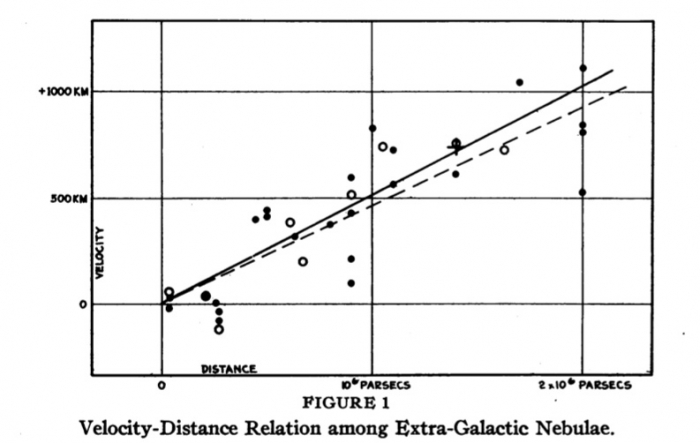
\includegraphics[width=\textwidth]{hubbleslaw}
        \caption{Hubbles Law}
        \label{fig:hubbleslaw}
\end{figure}

\begin{equation}\label{eq:hubble_law}
        \vb{v} = H_0 \vb{d},
\end{equation}

where $H_0$ is the \emph{Hubble constant}.
The observed \emph{redshifts} could not be explained by the proper motion of
the galaxies, instead this phenomenon was caused by the continuous expansion
of our Universe.

The expanding Universe was first theorized by Friedmann as a consequence of
the field equations of the theory of the \emph{General Relativity} (GR) in
1922, before Hubble's observations. The starting point of Friedmann
derivation was an elegant and powerful assumption about the structure of
our Universe: the \emph{Cosmological Principle}.

\subsection{The Cosmological Principle}\label{ss:cosmological_principle}

The matter in the Universe we observe is clustered in gravitationally bound
structures, but observations at large scale (\SI{> 100}{\mega\parsec}) shows
that the place we call home appears to obey the \emph{Cosmological
Principle}:

\begin{principle}[Cosmological Principle]
        On the largest scales, the Universe is spatially homogeneous and isotropic.
\end{principle}

Note that this principle is valid for every possible observer in the
universe. We see an homogeneous and isotropic universe from our point of
observation, and we believe that any other observer in the Universe does:
there's no special place in our Universe.

There are two main piece of evidence for the cosmological principle:

\begin{itemize}
        \item The \emph{Cosmic Microwave Background Radiation} (CMB): an almost
        uniform sea of photons which fills all space and provides a snapshot of the
        universe at \num{\sim 380000} years after its birth. The CMB
        presents small fluctuations in temperature and polarization with a
        characteristic scale:

        \begin{equation}
                \frac{\var{T}}{T} \leq \num{e-5}
        \end{equation}

        \item A relevant number of \emph{redshift surveys}, as the
        \emph{2dF Galaxy Redshift Survey} (2002); the \emph{Sloan Digital
        Sky Survey} (2007) and the \emph{Galaxy And Mass Assembly} survey
        (2008-2014), show that the distribution of stars looks increasingly
        smooth on larger scales.
\end{itemize}

\subsection{The FLRW Metric}\label{ss:flrw}

The acceptance of the cosmological principle provides a constraint to the
geometrical representation of the spacetime. There are several spacetime
metrics we can choose to describe the geometry of our Universe, but this
selection is reduced to those that adhere to the cosmological principle.

Friedmann, Lema\^itre, Robertson and Walker during the 1920-1930s proved
independently that the most generic metric based on the cosmological
principle is the Friedmann-Lema\^itre-Robertson-Walker (FLRW) metric:

\begin{equation}
        \dd{s}^2 = -c^2\dd{t^2} + a\qty(t)^2\qty[\dd{\chi}^2 +
        f_k\qty(\chi)^2\dd{\Omega}^2]
        \label{eq:flrw}
\end{equation}

Where:

\begin{itemize}
        \item $c$ is the speed of light in vacuum;
        \item $a\qty(t)$ is a real function of time known as \emph{scale factor};
        \item $k$ is a real number which parametrizes the spatial curvature of the
        spacetime. Due to the homogeneity and isotropy of space, $k$ is at most a
        function of time. For a fixed time $k$ is a constant and:

        \begin{itemize}
                \item $k = 0$ $\rightarrow$ flat universe;
                \item $k > 0$ $\rightarrow$ open universe;
                \item $k < 0$ $\rightarrow$ closed universe.
        \end{itemize}

        in particular:

        \begin{equation}
                f_k\qty(\chi) =
                        \begin{cases}
                                 \chi & \qif k = 0 \\
                                 \sqrt{k}^{-1} \sin(\sqrt{k} \chi) & \qif k > 0 \\
                                 \sqrt{\abs{k}}^{-1} \sinh(\sqrt{\abs{k}} \chi) & \qif k < 0
                        \end{cases}
        \end{equation}
        \item and $\dd{\Omega}^2 = \dd{\theta}^2 + \sin[2](\theta) \dd{\phi}^2$
        is the metric of the unitary sphere.
\end{itemize}

The FLRW metric in \autoref{eq:flrw} is invariant under the following transformation:

\begin{equation}
        \begin{split}
                \chi & \rightarrow \frac{\chi}{\lambda} \\
                k & \rightarrow \lambda k \\
                a & \rightarrow \lambda a
        \end{split}
\end{equation}

so it is possible to set:

\begin{align}
k & = 0,\pm 1 \\
a\qty(t_0) & = 1
\end{align}

where $t_0$ is the present time and the function $f_k$ becomes:

        \begin{equation}
                f_k\qty(\chi) =
                        \begin{cases}
                                 \chi & \qif k = 0 \\
                                 \sin \chi & \qif k = 1 \\
                                 \sinh \chi & \qif k = -1
                        \end{cases}
        \end{equation}

We can immediately note that the valid geometry for an homogeneous
and isotropic spacetime are either flat, spherical or hyperbolic.

\subsection{The Comoving Distance and the Hubble Parameter}

Although General Relativity allows one to formulate the laws of physics
using arbitrary coordinates, some coordinate choices are more natural or
easier to work with. \emph{Comoving coordinates} are an example of such a
natural coordinate choice.

Consider two points in a slice of space in the spacetime ($t = t_*$): $p_1$,
$p_2$. The physical distance between them is calculated using the FLRW
metric for a fixed time:

\begin{equation}
        \dd{s} = a\qty(t_*)\sqrt{\dd{\chi}^2 +
        f_k^2\qty(\chi)\dd{\Omega}^2}
\end{equation}

integrating between $p_1$ and $p_2$, we obtain:

\begin{equation}
        d_{\text{phys}} = a\qty(t_*)d_{\text{co}}
        \label{eq:dd}
\end{equation}

where $d_{\text{co}}$ is the comoving distance, the distance in comoving
coordinates, which expand in the same way as space, and $d_\text{phys}$ is
the proper or physical distance.

Taking the time derivative of \autoref{eq:dd}:

\begin{equation}
        v_{\text{phys}} = \dot a\qty(t) d_{\text{co}} = \frac{\dot a\qty(t)}{a\qty(t)} d_{\text{phys}}
\end{equation}

where $v_{\text{phys}}$ is the physical or proper velocity and the function:

\begin{equation}
        H\qty(t) = \frac{\dot a\qty(t)}{a\qty(t)}
        \label{eq:hubble_parameter}
\end{equation}

is called the \emph{Hubble parameter} and its present day value $H\qty(t_0)
\equiv H_0$ is the \emph{Hubble's constant}, introduced in
\autoref{ss:hubbleslaw}. The Hubble's constant is a cosmological
parameter of our standard cosmological model and has a positive value,
indicating that we live in an expanding universe.

\subsection{The Dynamics of Spacetime}

The time evolution of the FLRW metric, and thus the expansion rate of our
Universe, is determined by the evolution of the scale factor, $a\qty(t)$,
introduced in \autoref{ss:flrw}. On the other hand, the theory of General
Relativity provides a way to dynamically link the geometry of the spacetime
to the energy and momentum of matter and radiation present in the Universe.
Thus as expected, the evolution of the scale factor is governed by Einstein
field equations of GR:

\begin{equation}
        G_{\mu \nu} = \frac{8 \pi G}{c^2} T_{\mu \nu}
        \label{eq:einstein}
\end{equation}

where:

\begin{itemize}
        \item $G_{\mu \nu}$ is the Einstein tensor, which describes the
        geometry of the spacetime;
        \item $G$ is the universal gravitational constant;
        \item $T_{\mu \nu}$ is the energy-momentum tensor, responsible for
        the energy and momentum of matter.
\end{itemize}

Einstein fields equations of GR relate the geometry of the spacetime to the
distribution of matter within it. Assuming the cosmological principle, we
can choose $T_{\mu \nu}$ to be the energy-momentum tensor of a perfect
fluid, which can be completely characterized by its density and pressure:

\begin{equation}
         T_{\mu \nu} = (\rho c^2 + P)u_\mu u_\nu + P g_{\mu \nu}
         \label{eq:energy_momentum_tensor}
\end{equation}

Substituting \autoref{eq:flrw} and \autoref{eq:energy_momentum_tensor} in
\autoref{eq:einstein}, the field equations reduces to two equations for the
time evolution of the scale factor, known as \emph{Friedmann equations} and
written by Friedmann himself in 1922:

\begin{align}
        \qty(\frac{\dot a\qty(t)}{a\qty(t)})^2 & = \frac{8\pi G}{3} \rho\qty(t)
        - \frac{k\qty(t) c^2}{a^2\qty(t)}
        \label{eq:friedmann_1} \\
        \frac{\ddot a\qty(t)}{a\qty(t)} & = -\frac{4\pi G}{3}
        \qty(\rho\qty(t) + \frac{3 P\qty(t)}{c^2})
        \label{eq:friedmann_2}
\end{align}

The Friedmann equations constitutes a system of two differential equations
with three variables quantity: $a\qty(t)$, $\rho\qty(t)$ and $P\qty(t)$.
The last equation we need to close the system can be deduced from the
conservation of the energy-momentum tensor:

\begin{equation}
        \partial_\mu T^{\mu \nu} = 0
\end{equation}

It's the \emph{continuity equation}, which express the conservation of energy in a
cosmological setting:

\begin{equation}
        \dot \rho + 3 H \qty(\rho + \frac{P}{c^2}) = 0
        \label{eq:continuity}
\end{equation}

A state equation of the kind $P = P\qty(\rho)$ can be specified to
integrate the continuity equation and determine how the energy density
depends on the scale factor. We guess a generic and simple shape for the
state equation of each component of the cosmological fluid:

\begin{equation}
        P = w \rho c^2
        \label{eq:state}
\end{equation}

where $w$ is a parameter typical of each component.
Using \autoref{eq:state} in \autoref{eq:continuity} we obtain:

\begin{equation}
        \frac{\dot \rho}{\rho} = -3\qty(1 + w) \frac{\dot a}{a}
\end{equation}

integrating over time from $t_0$ to a generic time $t$ and using the fact
that $a\qty(t_0) = 1$:

\begin{equation}
        \rho_w\qty(t) = \rho_{w,0} a^{-3\qty(1 + w)}
\end{equation}

where $\rho_{0,w}$ is the present day energy density.
Therefore the total energy density for the cosmological fluid is:

\begin{equation}
        \rho_{\text{tot}} = \sum_w \rho_w
\end{equation}

and \autoref{eq:friedmann_1} becomes:

\begin{equation}
        H^2\qty(t) = \frac{8\pi G}{3} \rho_{\text{tot}}\qty(t) -
        \frac{k\qty(t) c^2}{a^2\qty(t)}
\end{equation}

where we have used \autoref{eq:hubble_parameter}. The curvature parameter
$k$ can isolated in the right-hand side of the equation:

\begin{equation}
        \begin{split}
                \frac{k\qty(t) c^2}{a^2\qty(t)} & =
                \frac{8\pi G \rho_{\text{tot}}\qty(t)}{3} - H^2\qty(t) \\
                \frac{k\qty(t) c^2}{a^2\qty(t)} & =
                H^2\qty(t) \qty(\frac{8\pi G \rho_{\text{tot}}\qty(t)}{3H^2\qty(t)} - 1) \\
                k(t) & = \frac{H^2\qty(t) a^2\qty(t)}{c^2} \qty(\Omega\qty(t) - 1) \\
        \end{split}
        \label{eq:friedmann_curvature}
\end{equation}

In the last equation we have defined:

\begin{align}
        \rho_c\qty(t) & \equiv \frac{3H^2\qty(t)}{8\pi G} \\
        \Omega\qty(t) & \equiv \frac{\rho_{\text{tot}}\qty(t)}{\rho_c\qty(t)}.
\end{align}

The function $\rho_c\qty(t)$ is known as the \emph{critical density}: it
represents the energy density time evolution for a flat universe ($k = 0$).
We note that in this case, the total energy density of the Universe is
directly related to the Hubble parameter.

Evaluating \autoref{eq:friedmann_curvature} for $t = t_0$ and assuming a
time independent space curvature $k(t) = k$, yields:

\begin{equation}
        k = \frac{H^2_0}{c^2} \qty(\Omega_0 - 1) \\
\end{equation}

where:

\begin{equation}
        \Omega_0 \equiv \frac{\rho_0}{\rho_{c,0}} = \sum_w
        \frac{\rho_{w,0}}{\rho_{c,0}} \equiv \sum_w \Omega_w
\end{equation}

The adimensional quantities $\Omega_w$ are the \emph{density parameters}
for each fluid component. Note that even though we have omitted the $0$
subscript, the density parameters refer to the fraction of energy observed
today, as the definition implies.

The density parameters sum to:

\begin{equation}
        \sum_w \Omega_w = 1 + \frac{kc^2}{H^2_0}
\end{equation}

as a consequence, if we live in a flat universe then we must have $\sum_w
\Omega_w = 1$. Any excess energy density, with $\sum_w \Omega_w > 1$ means
that we necessarily live in a positively curved universe with $k = +1$. Any
deficit in energy, with $\sum_w \Omega_w < 1$ gives rise to a negatively
curved $k = 1$ universe. Measuring the present day total energy density
$\rho_{\text{tot},0}$ and the Hubble constant $H_0$, gives us the
opportunity to have knowledge of the spatial geometry of our Universe.

\subsection{The Components of the Cosmological Fluid}

According to current theories and pieces of evidence, there are three
entities that contribute to the current energy density of our Universe:
conventional matter or \emph{dust}; radiation and Dark Energy or
\emph{cosmological constant}.
To derive a solution for the time evolution of the scale factor $a\qty(t)$
in our Universe, it is essential to write a state equation
$P\qty(\rho) = \rho$ for each one of these component:

\begin{itemize}
        \item For dust-like matter (e.g. galaxies or cold dark matter):
        $P_m\qty(\rho_m) = 0$;
        \item For radiation we must impose a null trace for the energy-momentum
        tensor $T_{\mu \nu}$ in \autoref{eq:energy_momentum_tensor}: $P_r\qty(\rho_m)
        = \rho_r c^2/3$;
        \item For Dark Energy the equation of state is obtained
        substituting  $G_{\mu \nu} = -g_{\mu \nu} \Lambda$, with $\Lambda =
        \text{const.}$ and $\Lambda > 0$, in \autoref{eq:einstein}:
        $P_\Lambda\qty(\rho_\Lambda) = -\rho_\Lambda c^2$, $\rho_\Lambda =
        \Lambda/8\pi G$.
\end{itemize}

The dependence on the scale factor for the energy densities characterized by
these state equations is found making use of the continuity equation
(\autoref{eq:continuity}):

\begin{align}
        \rho_m\qty(a) & = \rho_{m,0}a^{-3} \label{eq:rho_m} \\
        \rho_r\qty(a) & = \rho_{r,0}a^{-4} \label{eq:rho_r} \\
        \rho_\Lambda\qty(a) & = \rho_{\Lambda,0} \label{eq:rho_lambda}. \\
\end{align}

The quantity $\Lambda$ is known as the \emph{cosmological constant} and the
corresponding density $\rho_\Lambda$ is the \emph{vacuum energy density},
associated with the \emph{zero-point energy} of the vacuum state. Note that
Dark Energy has negative pressure $P_\Lambda = -\rho_\Lambda c^2$, and it
does not dilute away as the Universe expands.

The total energy density of our Universe is:

\begin{equation}
        \rho_\text{tot}\qty(a) = \frac{\rho_{m,0}}{a^3} + \frac{\rho_{r,0}}{a^4} +
        \rho_{\Lambda,0}.
\end{equation}

An expanding universe is radiation dominated at first, in a second phase
its expansion is driven by matter and at last by Dark Energy. In fact every
universe characterized by a non-zero cosmological constant ($\Lambda \neq
0$) will be ultimately become dominated by the vacuum energy density
$\rho_\Lambda$. A plot of the evolution of the three kinds of energy
density is shown in \autoref{fig:density_evolution}.

\begin{figure}
        \centering
        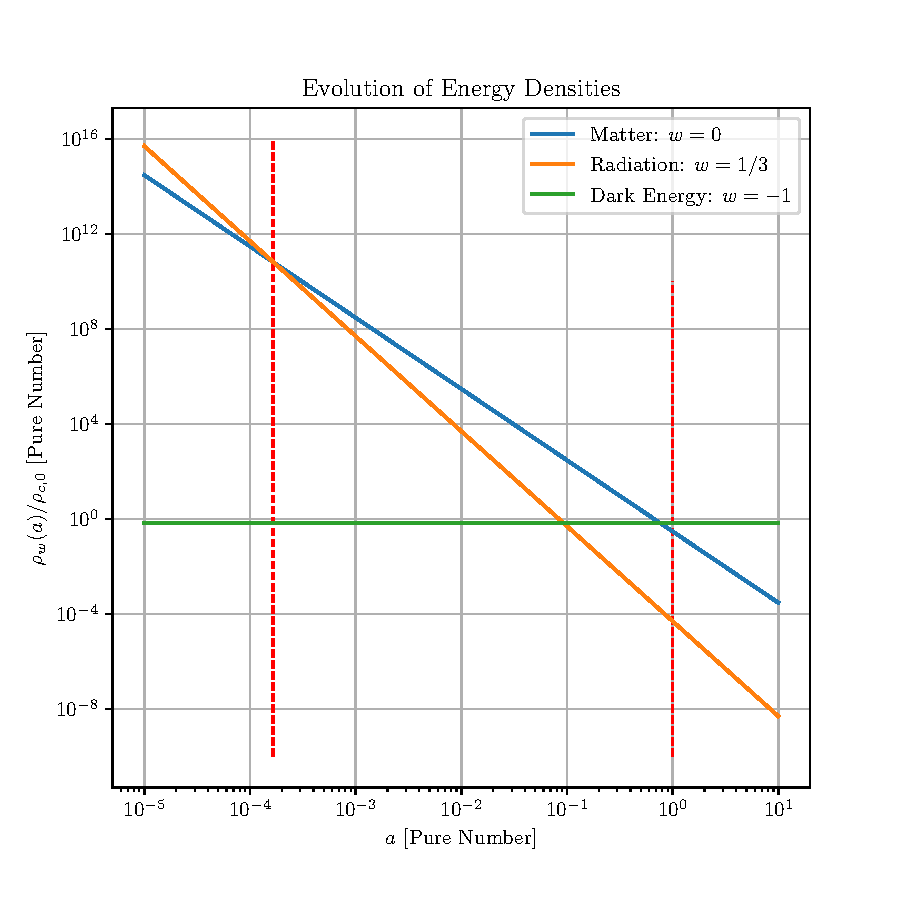
\includegraphics[width=\textwidth]{density_evolution}
        \caption{Energy density evolution.}
        \label{fig:density_evolution}
\end{figure}

Given the total energy density we can solve the first Friedmann equation
and obtain the evolution of the scale factor in our Universe. The scale
factors for the three different space curvatures ($k = 0,\pm 1$) in the
simple case of a matter dominated universe are sketched in
\autoref{fig:scale_factor_evolution_matter}. In the case of an expanding
flat or hyperbolic geometry ($k = 0,-1$) the Universe expands for ever with:

\begin{equation}
        \dot a\qty(t \rightarrow +\infty)
                \begin{cases}
                        > 0 & \qif k = -1 \\
                        \rightarrow 0 & \qif k = 0
                \end{cases}
\end{equation}

The spherical universe ($k = +1$) instead eventually re-collapses at a finite
time $t_{\text{bc}}$ with:

\begin{equation}
        a\qty(t_{\text{bc}}) = 0
\end{equation}

This event is known as \emph{Big Crunch}.

\begin{figure}
        \centering
        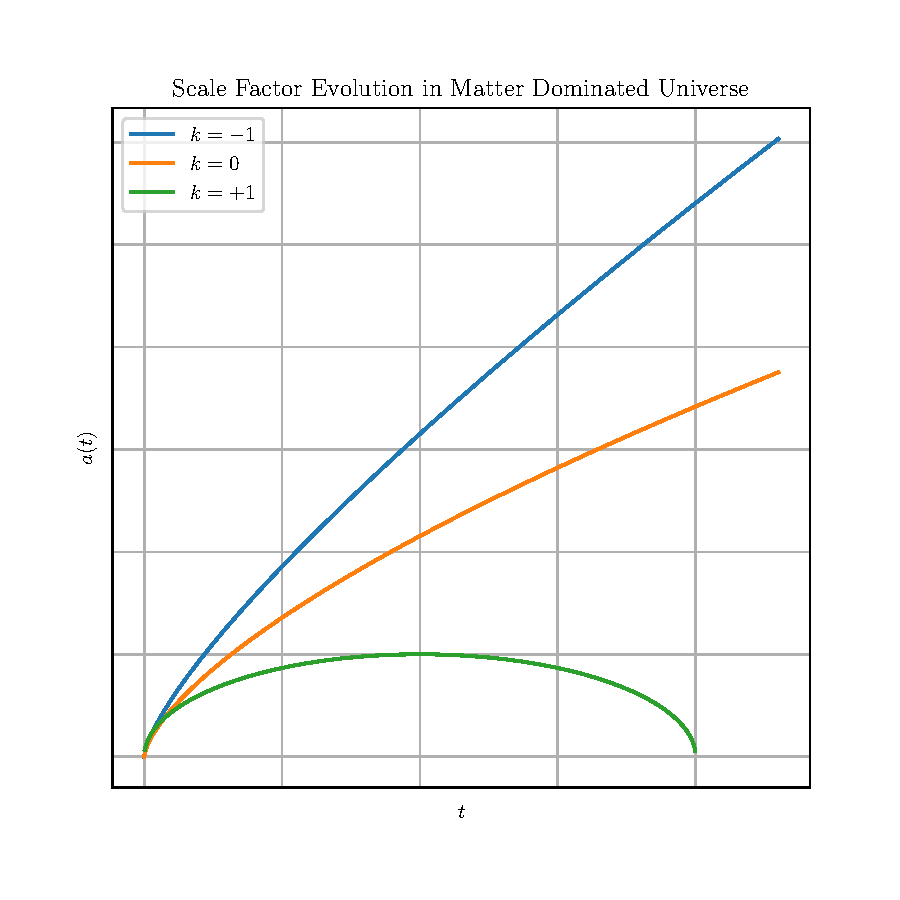
\includegraphics[width=\textwidth]{scale_factor_evolution_matter}
        \caption{Scale factor evolution in a matter dominated universe.}
        \label{fig:scale_factor_evolution_matter}
\end{figure}

In the case of Dark Energy dominated universe every possible solution for
each one of the three space curvatures describes the same spacetime, but with
different coordinates. This spacetime is known as \emph{de Sitter space}.
The evolution of the scale factor for this kind of universe is shown in
\autoref{fig:scale_factor_evolution_sitter}. This solution shows a
contracting phase when $t < 0$, followed by a phase of accelerating
expansion ($\ddot a > 0$) when $t > 0$. In particular there's no
\emph{Big Bang} when $t = 0$:

\begin{equation}
        a\qty(t = 0) = \sqrt{\frac{3c^2}{\Lambda}}
\end{equation}

\begin{figure}
        \centering
        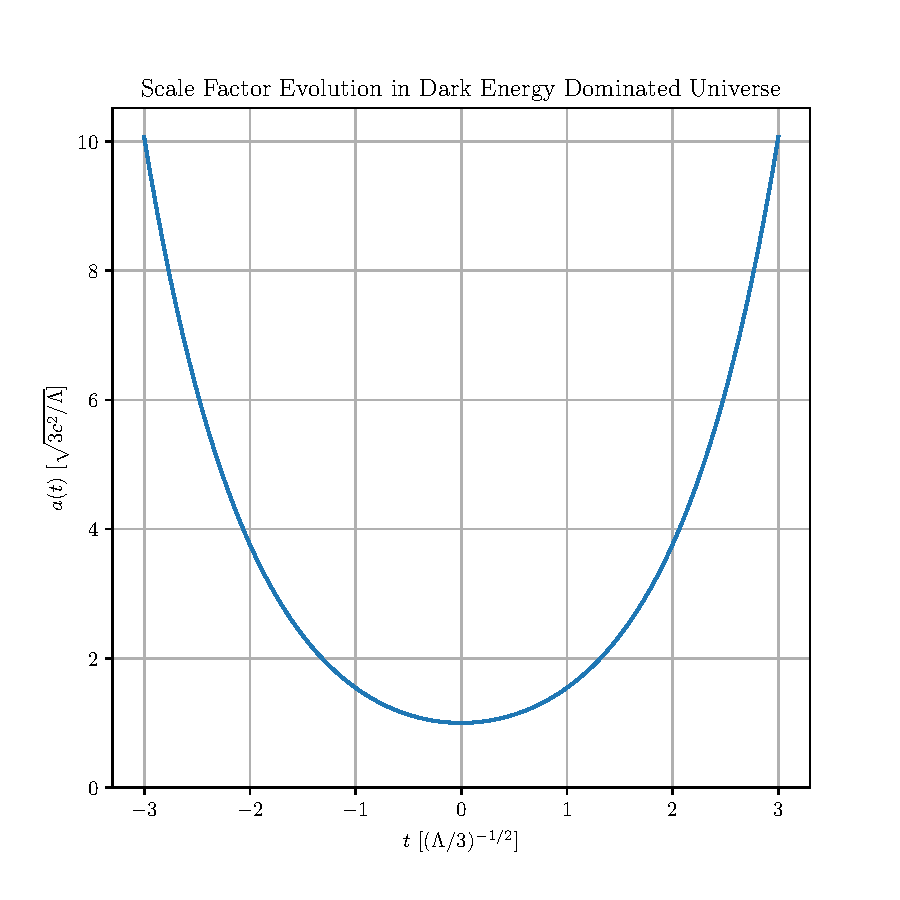
\includegraphics[width=\textwidth]{scale_factor_evolution_sitter}
        \caption{Scale factor evolution for de Sitter space}
        \label{fig:scale_factor_evolution_sitter}
\end{figure}

\subsection{The \texorpdfstring{$\Lambda$}{LAMBDA-}CDM Cosmological Model}

Substituting the expressions for the energy densities of the components of
the cosmological fluid (\autoref{eq:rho_m}, \autoref{eq:rho_r} and
\autoref{eq:rho_lambda}) in \autoref{eq:friedmann_1} yields the second
Friedmann equation for our Universe:

\begin{equation}
        H^2\qty(t) = \frac{8\pi G}{3} \qty(\frac{\rho_{m,0}}{a^3\qty(t)} +
        \frac{\rho_{r,0}}{a^4\qty(t)} + \rho_{\Lambda,0}) -
        \frac{k\qty(t) c^2}{a^2\qty(t)}
\end{equation}

If the first term in the right-hand side is multiplied and
divided by the squared hubble constant $H^2_0$, the equation is parametrized
by the density parameters $\Omega_w$:

\begin{equation}
        H^2\qty(t) = H^2_0 \qty(\frac{\Omega_m}{a^3\qty(t)} +
        \frac{\Omega_r}{a^4\qty(t)} + \Omega_\Lambda) -
        \frac{k\qty(t) c^2}{a^2\qty(t)}
\end{equation}

The collection of the numbers $\Omega_m$, $\Omega_r$, $\Omega_\Lambda$ and
$k$ goes by the name of the \emph{$\Lambda$CMD model}, with $\Lambda$
denoting the cosmological constant and CMD denoting \emph{cold dark matter}.
The great interest in the study of the Cosmic Microwave Background resides
in the fact that the values of the parameters of the $\Lambda$CMD
cosmological model can be extracted from observations of this relic
radiation.

\section{The CMB Radiation}

This section is devoted to the introduction of the Cosmic Microwave
Background (CMB) Radiation. To understand what caused the presence of the
cosmic microwave background radiation, we start describing
what we think happened in the Universe from the first instants after the
Big Bang to today.

\subsection{A Brief Thermal History of Our Universe}\label{ss:brief_thermal_history}

The essence of the hot Big Bang theory is simply to go back in time taking
the temperature scaling $T \sim 1/a$. As the solution for the scale
factor suggests, as we go further back in time, more the temperature and
the energy density of the Universe increase and more species join the
primordial plasma reaching the thermodynamic equilibrium. As we know in the
early stages the Universe was radiation dominated, so the temperature and
energy density decreased according to:

\begin{equation}
        T\qty(t), \rho\qty(t) \propto t^{-\frac{1}{2}}
\end{equation}

A summary of some of the key events in the early history of the Universe
follows:

\begin{itemize}
        \item \textbf{Electroweak phase transition:} \SI{e-12}{\second},
        \SI{e22}{\kelvin}

        At this time the electroweak phase transition occurred, separating
        the weak and electromagnetic interactions. In this epoch the
        universe was filled with a quark-gluon plasma.
        \item \textbf{QCD phase transition:} \SI{e-6}{\second},
        \SI{e16}{\kelvin}

        At this time the average energy of particles interaction had fallen
        below the mass of the hadrons. In this epoch the temperature was
        high enough that hadrons and anti-hadrons pairs could form. Later
        new pairs were no longer produced and most of the hadrons and
        anti-hadrons annihilated. Due to the matter and anti-matter
        asymmetry a small portion of hadrons remained in the Universe.

        At this time the Universe was filled with neutrons and protons in
        the ratio of:

        \begin{equation}
                \frac{n_n}{n_p} = \frac{1}{5}
        \end{equation}

        due to the small mass difference between the two particles. Later
        this ratio became smaller as a consequence of the neutron $\beta$
        decay:

        \begin{equation}
                n \rightarrow p + e^- + \bar\nu_e
        \end{equation}

        and its present day value is:

        \begin{equation}
                \frac{n_n}{n_p} = \frac{1}{7}
        \end{equation}

        \item \textbf{Neutrino Decoupling:} \SI{1}{\second},
        \SI{e10}{\kelvin}

        At this time neutrinos decoupled from the primordial plasma and
        began to travel freely into space. As neutrinos rarely interact
        with matter, they still exist today as the Cosmic
        Neutrino Background (C$\nu$B), analogous to the much later Cosmic
        Microwave Background emitted during recombination.

        \item \textbf{$e^-e^+$ Annihilation:} \SI{6}{\second},
        \SI{5e9}{\kelvin}

        At this time the average energy of photons became less then the rest mass
        of the electron-positron pairs and the reaction:

        \begin{equation}
                2\gamma \rightleftharpoons e^- + e^+
        \end{equation}

        fell out of equilibrium. The left $e^-e^+$ pairs annihilated and,
        due to the matter and anti-matter asymmetry, just a small portion
        of electrons survived.

        \item \textbf{Nucleosynthesis:} \SI{3}{\minute}, \SI{e9}{\kelvin}

        At this time the temperature and pressure of the Universe allowed
        the stabilization of deuterium and the consequent formation of
        light nuclei, such as hydrogen and its isotopes
        (\SI{\sim 75}{\percent}) and helium (\SI{\sim 25}{\percent}).

        \item \textbf{Matter-Radiation Equality:} \SI{50000}{\year},
        \SI{8700}{\kelvin}

        At this time the Universe became matter dominated: the energy
        density of matter $\rho_m$ became equal to the energy density of
        radiation $\rho_r$ (\autoref{fig:density_evolution}).

        \item \textbf{Recombination and Last Scattering:} \SI{370000}{\year},
        \SI{3000}{\kelvin}

        At this time the Universe has cooled enough ($k_bT <<
        \SI{13.6}{\electronvolt}$) to allow the formation of the first
        neutral atoms. This event is known as \emph{recombination} and it is
        associated to the photons decoupling or \emph{last scattering}, that
        refers to the mean free path of photons in the Universe becoming
        infinite. Nowadays the last scattering photons are still propagating in
        space and we refer to them as the \emph{Cosmic Microwave Background}.

        \item \textbf{Matter-Dark Energy Equality:} \SI{e10}{\year},
        \SI{3.8}{\kelvin}

        At this time the Universe became dominated by Dark Matter: the
        vacuum energy density $\rho_\Lambda$ became equal to the energy density of
        matter $\rho_m$ (\autoref{fig:density_evolution}), determining a
        phase of accelerated expansion.

        \item \textbf{Today:} \SI{1.38e10}{\year}, \SI{2.7}{\kelvin}

        Previously we have referred to this time as $t_0$: this is
        the epoch we live in. Currently the Universe remains dominated by
        Dark Energy, it is undergoing and will continue to undergo an exponential
        expansion.
\end{itemize}

\subsection{The First Revelation of the CMB}

The Cosmic Microwave Background was first predicted in 1984 by Ralph Alpher
and Robert Herman, who also provided a first estimation of its brightness
temperature (\SI{\sim 5}{\kelvin}).

Andrew McKellar in 1941 used spectroscopic observations of the cyano radical
absorption lines in star spectra to detect a rotational temperature of
interstellar molecules. However McKellar failed to provide a cosmological
interpretation for these observations.

In 1964 Arno Penzias and Robert Wilson were working at Bell Laboratories
on a microwave horn antenna (\autoref{fig:horn_antenna_pw}) originally used by
the Bell telephone companies for satellite communication.
To their surprise they found a background noise which did not depend on the
direction, with a temperature that they measure to be between
\SI{2.5}{\kelvin} and \SI{4.5}{\kelvin}. They were observing the CMB
radiation and for this discovery they were awarded the Nobel Prize in 1978.

\begin{figure}
        \centering
        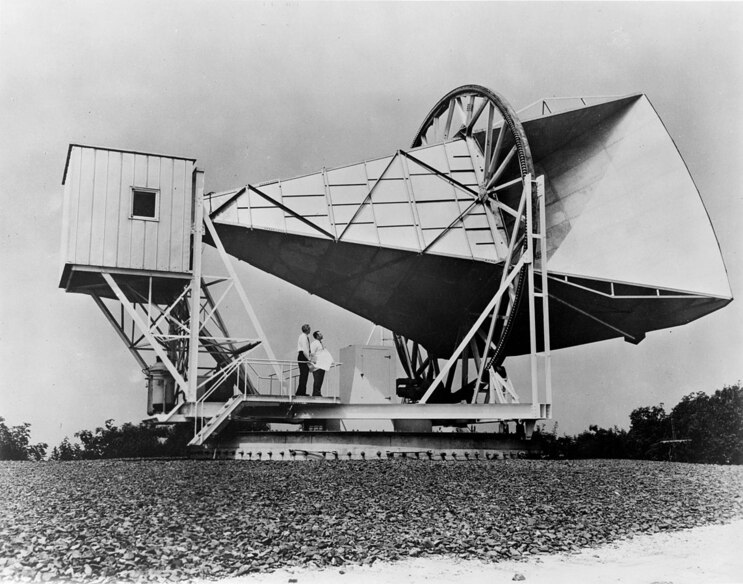
\includegraphics[width=\textwidth]{Horn_Antenna_PW}
        \caption{Penzias and Wilson's microwave horn antenna.}
        \label{fig:horn_antenna_pw}
\end{figure}

\subsection{The CMB Black Body Spectrum}\label{ss:cmb_bb}

Just before recombination and last scattering photons were
coupled with matter and in thermodynamic equilibrium. The spectral density
of electromagnetic radiation in thermodynamic equilibrium is described by
the \emph{Planck law}:

\begin{equation}
        B_\nu\qty(T) = \frac{2h\nu^3}{c^2}
        \frac{1}{\exp(\frac{h\nu}{K_b T}) - 1}
\end{equation}

where $T$ is the temperature of the thermal bath, $\nu$ is the frequency of
the electromagnetic radiation, $K_b$ is the Boltzmann constant and $h$ is
the quantum of action, the Planck constant. As mentioned in
\autoref{ss:brief_thermal_history}, at recombination the temperature of the
universe was \SI{\sim 3000}{\kelvin}, therefore, making use of the Wien
Law:

\begin{equation}
        \lambda_{\text{peak}} = \frac{b}{T}
\end{equation}

where $b \approx \SI{2.897e-3}{\meter\kelvin}$ and
$\lambda_{\text{peak}}$ is the wavelength at which the spectrum
peaks, we know that at recombination:

\begin{equation}
        v_{\text{CMB,max}} \approx \SI{7e4}{\giga\hertz}
\end{equation}

As we stated in \autoref{ss:brief_thermal_history}, the temperature of the
universe is related to the scale factor

\begin{equation}
        T\qty(a) \propto \frac{1}{a}
\end{equation}

and as a consequence

\begin{equation}
        T\qty(a_0) = T\qty(a_{\text{rec}}) a_{\text{rec}}
        \label{eq:t_scale}
\end{equation}

where $a_{\text{rec}}$ is the scale factor at the time of recombination.

At the same time, the photons of the CMB radiation are affected by \emph{cosmological
redshift}, due to Universe expansion. The wavelength of the light emitted
at the time of recombination differs from the light observed at present
time, according to the law

\begin{equation}
        \lambda\qty(a_0) = \frac{\lambda\qty(a_{\text{rec}})}{a_{\text{rec}}}.
\end{equation}

For frequency this translates to

\begin{equation}
        \nu\qty(a_0) = \nu\qty(a_{\text{rec}}) a_{\text{rec}}
        \label{eq:nu_scale}
\end{equation}

and, if we combine \autoref{eq:t_scale} and \autoref{eq:nu_scale}, we
obtain:

\begin{equation}
        \frac{h \nu\qty(a_0)}{K_b T\qty(a_0)} =
        \frac{h \nu\qty(a_{\text{rec}})}{K_b T\qty(a_{\text{rec}})}.
\end{equation}

This last equation asserts that the shape of the CMB spectrum does not
change as the Universe expands. However, the characteristic temperature and
peak frequency of the spectrum have changed according to
\autoref{eq:t_scale} and \autoref{eq:nu_scale}, so that

\begin{align}
        T_{\text{CMB}} & \approx \SI{3000}{\kelvin} a_{\text{rec}} \approx
        \SI{3}{\kelvin} \\
        v_{\text{CMB,max}} & \approx \SI{7e4}{\giga\hertz} a_{\text{rec}}
        \approx \SI{70}{\giga\hertz}
\end{align}

The spectrum of the CMB was measured with high accuracy
(see \autoref{fig:cmb_spectrum_cobe})
by the \emph{Far infrared Absolute Spectrometer} (FIRAS) instrument onboard
the \emph{Cosmic Background Explorer} (COBE) satellite: it is a near
perfect black body spectrum at $T = \SI{2.7260 \pm 0.0013}{\kelvin}$

\begin{figure}
        \centering
        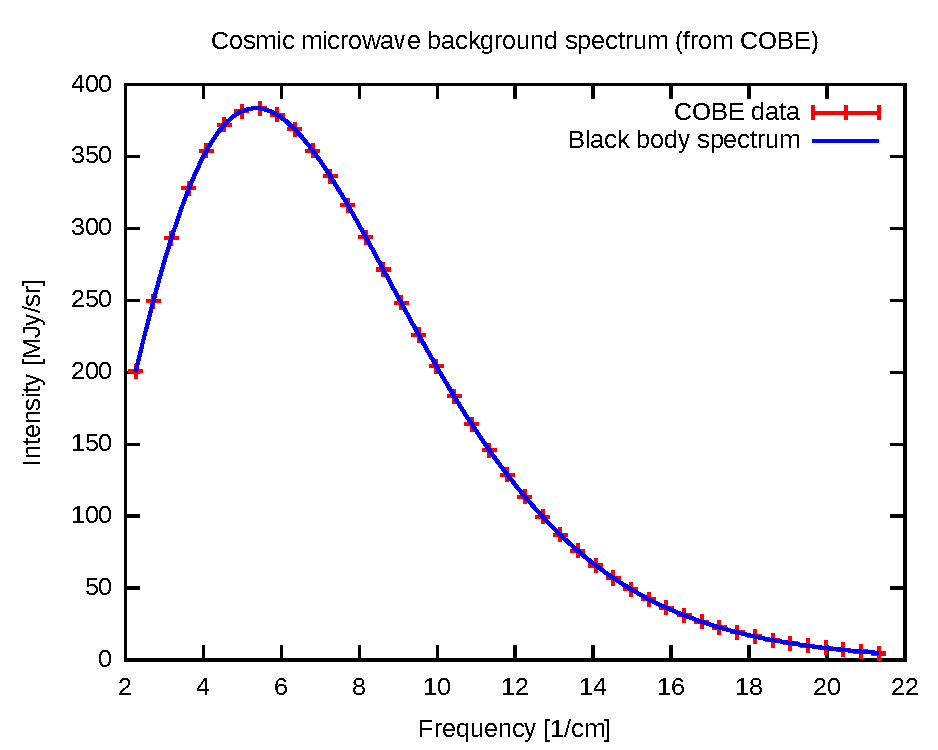
\includegraphics[width=\textwidth]{CMB_Spectrum_COBE}
        \caption{CMB Spectrum COBE}
        \label{fig:cmb_spectrum_cobe}
\end{figure}

\section{The CMB Temperature Anisotropies}

The CMB radiation is extremely isotropic. As mentioned in
\autoref{ss:cosmological_principle} the temperature anisotropies are of the
order of

\begin{equation}
\frac{\Delta T\qty(\theta,\phi)}{\bar T} \sim \num{e-5}
\end{equation}

for every $\theta$ and $\phi$ on the sky, $0 \leq \theta \leq \pi$,
$0 \leq \phi \leq 2\pi$.

Sachs and Wolfe in 1967 had theorized first the presence of temperature
anisotropies in the CMB spectrum at large angular scales. Later
anisotropies were linked to the quantum oscillations in primordial plasma,
but the instruments used before the 90s were not sensible enough to carry
out useful measures of this phenomenon.

The \emph{Differential Microwave Radiometer} (DMR) instrument onboard the
COBE satellite was the first experiment to map the CMB temperature
anisotropies.The instrument consists of six differential microwave
radiometers, two nearly independent channels that operate at each of three
frequencies: \SI{ 31.5}{\giga\hertz}, \num{53}, and \SI{90}{\giga\hertz}.
Making use of two years of DMR data, the amplitude of temperature fluctuations
was reported to be
\SI{36 \pm 5}{\micro\kelvin} at \ang{7}, and
\SI{30.5 \pm 2.7}{\micro\kelvin} when smoothed to \ang{10}.
\autoref{fig:dmr_maps} represents DMR data from the \SI{53}{\giga\hertz}
band on a scale from \SIrange{0}{4}{\kelvin}, showing the near-uniformity of the
CMB brightness, on a scale intended to enhance the contrast due to
the dipole anisotropy, and following subtraction of the dipole component.

\begin{figure}
        \centering
        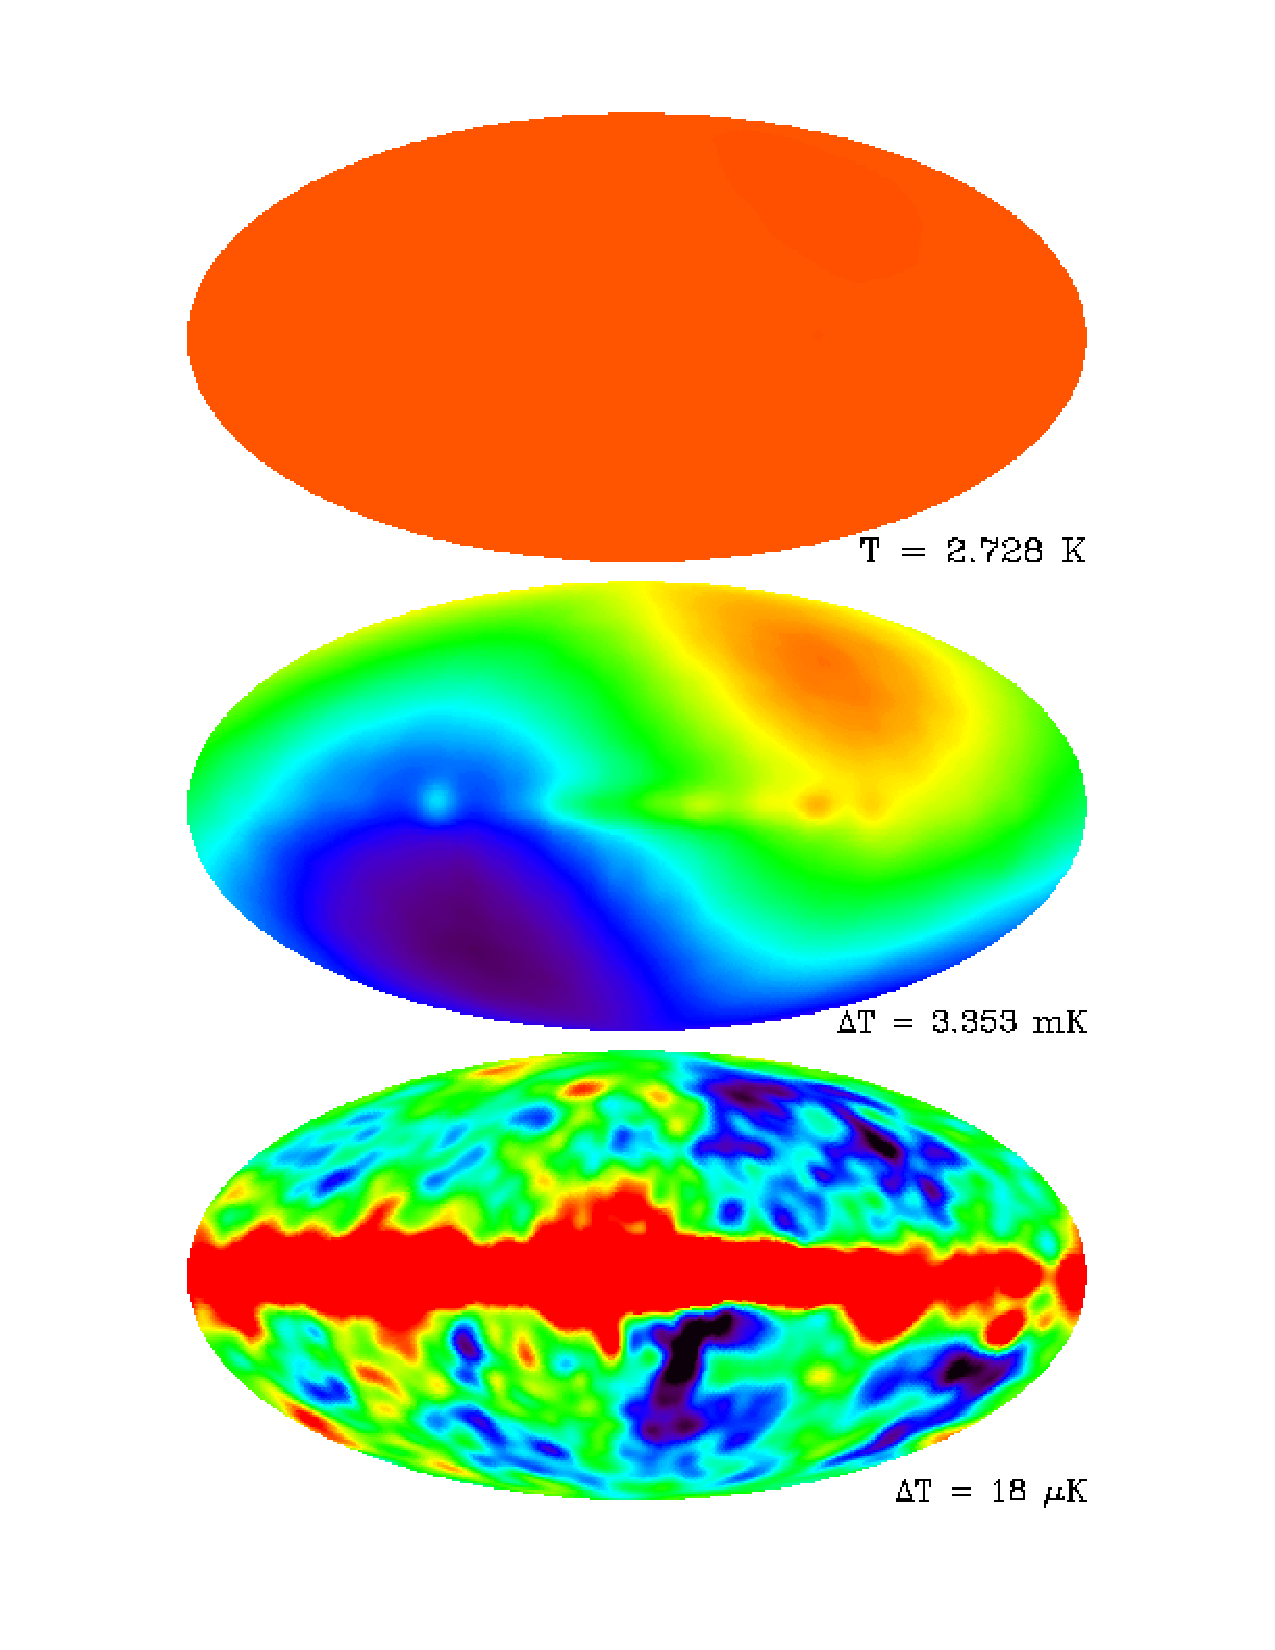
\includegraphics[width=0.90\textwidth]{DMR_maps_2.pdf}
        \caption{COBE-DMR CMB anisotropies sky maps.}
        \label{fig:dmr_maps}
\end{figure}

The second generation of CMB experiments was represented by the
\emph{Wilkinson Microwave Anisotropy Probe} (WMAP). The WMAP mission was
designed to acquire a \ang{;13;} FWHM resolution full sky
map of the temperature anisotropy of the cosmic microwave background
radiation. WMAP observed the microwave sky for \num{9} years in \num{5}
bands. The skymap data products derived from the WMAP observations have
\num{45} times the sensitivity and \num{33} times the angular resolution
of the COBE-DMR mission.

\emph{Planck} was the third generation of space-based cosmic microwave background
experiments, after NASA's COBE and NASA's WMAP. It was also the third
Medium-Sized Mission (M3) of European Space Agency's (ESA's) Horizon 2000
Scientific Program. The basic scientific goal of the Planck mission is to
measure CMB anisotropies at all angular scales larger than \ang{;10;}
over the entire sky with a precision of \num{\sim 2} parts per million.
The model payload consisted of a \SI{1.5}{\meter} off-axis telescope with
two focal plane arrays of detectors sharing the focal plane. Low frequencies
were covered by \num{56} tuned radio receivers sensitive to
\SIrange{30}{100}{\giga\hertz}, while high frequencies were be covered by
\num{56} bolometers sensitive to \SIrange{100}{850}{\giga\hertz}.
The Planck mission permitted the extraction of the most precise map of the
CMB temperature anisotropies, to date. This map is depicted in
\autoref{fig:planck_cmb}.

\begin{figure}
        \centering
        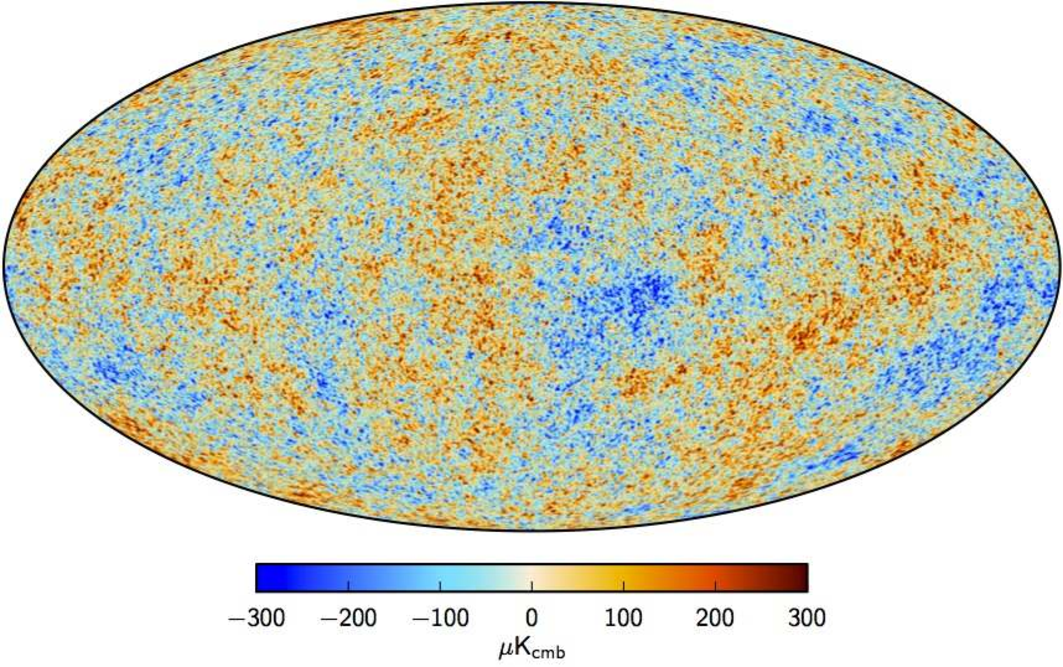
\includegraphics[width=\textwidth]{Planck_CMB}
        \caption{CMB Anisotropies Planck}
        \label{fig:planck_cmb}
\end{figure}

A comparison of the results obtained by COBE, WMAP, and Plank is showed in
\autoref{fig:cobe_wmap_planck_comparison}.

\begin{figure}
        \centering
        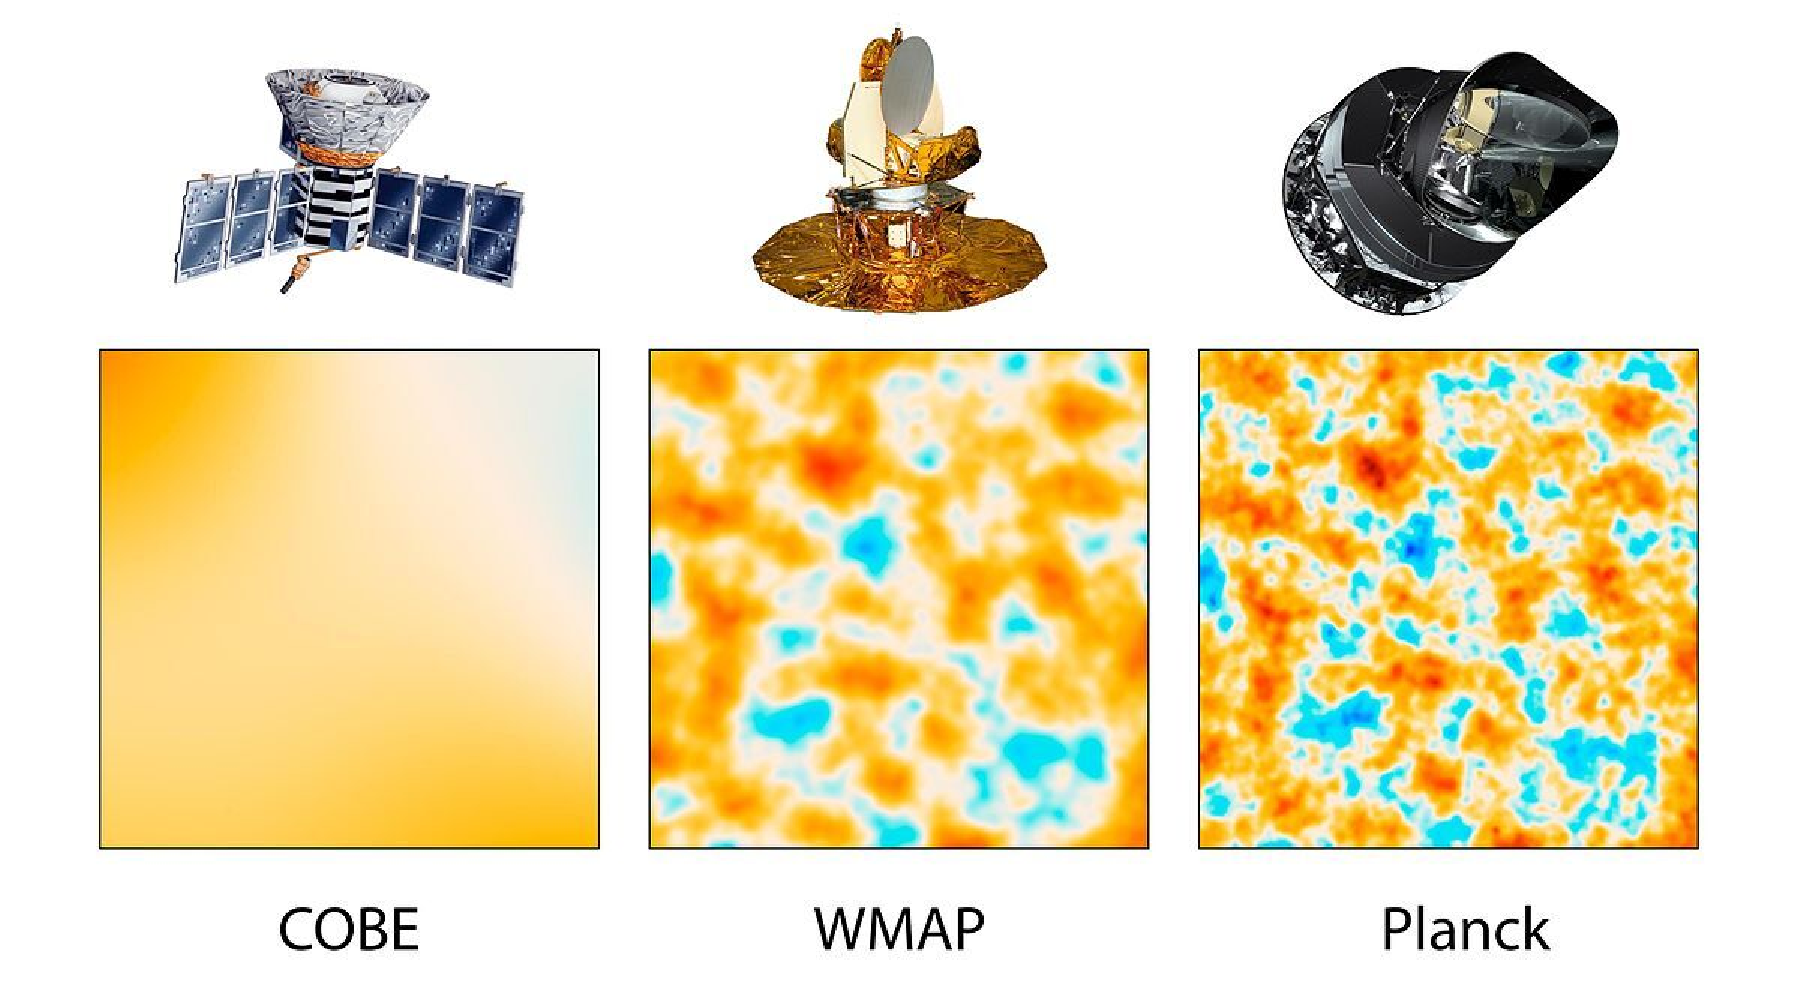
\includegraphics[width=\textwidth]{cobe_wmap_planck_comparison}
        \caption{COBE, WMAP, and Plank results comparison.}
        \label{fig:cobe_wmap_planck_comparison}
\end{figure}

\subsection{Density Fluctuations}

The CMB radiation anisotropies contain an imprint of the anisotropies at
the time of recombination and, if traced back in time, they can be
interpreted as a signature of the perturbations in the primordial plasma.
Precise measures of the CMB anisotropies pattern let us discriminate
between different cosmological models.

The perturbations in the early universe were adiabatic, that is, the
perturbations in all components of the cosmological fluid are proportional.
In particular

\begin{equation}
        \delta_r\qty(\vb{\chi},t) \equiv \frac{4}{3} \delta_m\qty(\vb{\chi},t)
\end{equation}

where $\delta_x\qty(\vb{\chi},t)$ is the \emph{density contrast} for a
specific component of the cosmological fluid

\begin{equation}
        \delta_x\qty(\vb{\chi},t) = \frac{\var{\rho_x\qty(\vb{\chi},t)}}{\bar \rho_x}
\end{equation}

$\bar \rho_x$ is the average density.

We express the adiabatic relation between radiation and matter in terms of
temperature fluctuation in the CMB. The Stefan-Boltzmann law, which is
valid for a black body, states that

\begin{equation}
        I = \sigma T^4
\end{equation}

where I is the intensity of radiant energy, and $\sigma$ is the
Stefan-Boltzmann constant. We deduce that $\rho_r \sim T^4$, so

\begin{equation}
        \delta_r = 4 \frac{\var{T}}{\bar T}.
\end{equation}

As a consequence of the adiabatic nature of the primordial density
perturbations, we conclude that

\begin{equation}
        \frac{\var{T}}{\bar T} = \frac{1}{3} \delta_m.
\end{equation}

It is best to perform the Fuorier transform of the density contrast

\begin{equation}
        \delta \qty(\vb{k},t) = \int \dd[3]{\vb{\chi}} e^{i\vb{k} \vdot
        \vb{\chi}} \delta\qty(\vb{\chi},t)
\end{equation}

because the comoving wavenumber $k = a\qty(t) k_\text{phys}$ is linked to a
physical scale represented by the physical wavelength

\begin{equation}
        \lambda_\text{phys} = \frac{2\pi a\qty(t)}{k}.
\end{equation}

In the hypothesis  of a flat universe ($k = 0$), the wave modes of the
primordial density contrast $\delta\qty(\vb{k},t = t_\text{BigBang})$
has evolved over time since Big Bang, according to the perturbation
equation. Such equation is obtained linearising the fluid equations
for a perfect fluid in an expanding spacetime:

\begin{equation}
        \ddot \delta\qty(\vb{\chi},t) + 2H\qty(t)\dot \delta\qty(\vb{\chi},t) -
        c_s^2\qty(1 + w)\qty(\frac{1}{a^2\qty(t)} \laplacian_\chi + \qty(
        1 + w)k^2_j)
        \delta\qty(\vb{\chi},t) = 0
\end{equation}

which in Fourier space become

\begin{equation}
        \ddot \delta\qty(\vb{k},t) + 2H\qty(t)\dot \delta\qty(\vb{k},t) -
        c_s^2\qty(1 + w)\qty(\frac{k^2}{a^2\qty(t)} + \qty(1 + w)k^2_j)
        \delta\qty(\vb{k},t) = 0.
        \label{eq:perturbations_density}
\end{equation}

The relevant quantities in the last equation are:

\begin{itemize}
        \item $c_s$: the speed of sound for the fluid;
        \item $k_J$: the \emph{Jeans wavenumber}, which is related to the
        \emph{Jeans length scale}

        \begin{equation}
                \lambda_J = c_s c \sqrt{\frac{\pi}{G \bar \rho}}.
        \end{equation}

        Only modes with $\lambda > \lambda_J$ will grow over time. This is
        known as \emph{Jeans instability}.
        For modes with $\lambda < \lambda_J$
        \autoref{eq:perturbations_density} is that of a damped harmonic
        oscillator, so this modes does not grow.

        \item $w$: the same parameter that appears in the equation of state
        for a specific component of the cosmological fluid

        \begin{equation}
                P\qty(t) = w \rho\qty(t) c^2.
        \end{equation}
\end{itemize}

The other relevant scale length, in addition to the Jeans length scale is
set by the expansion of the Universe,

\begin{equation}
        d_H \approx cH^{-1} = c^2 \sqrt{\frac{3}{8\pi G \bar \rho}}.
\end{equation}

This is known as the \emph{apparent horizon} or \emph{Hubble radius}.
Each Fourier mode of a perturbation
is a coherent wave and causality prohibits the formation of such perturbations
in case of $\lambda > d_H$, since there is no time for information to cross
this distance since the Big Bang.

We know that at recombination our Universe was matter dominated, so

\begin{align}
        a\qty(t) & \propto t^\frac{2}{3} \\
        H\qty(t) & = \frac{2}{3t}.
\end{align}

In principle we can substitute these expressions into
\autoref{eq:perturbations_density} and derive a solution for each component
of the cosmological fluid and each wavelength, studying if it lays inside
or outside the apparent horizon and within the Jeans scale length.

There is a subtlety to consider, if we want to extend this line of reasoning
to the temperature contrast. Photons, to reach an observer from any point
in space $\vb{x}$, must escape the gravitational potential. During this
process they lose energy and so they are redshifted. This effect is known
as \emph{gravitational redshift}. This change in energy density in turn
shifts the temperature fluctuations in the CMB. If we consider a varying
gravitational potential $\delta \phi\qty(\vb{\chi})$, then we obtain

\begin{equation}
        \frac{\var{T\qty(\vu{n})}}{\bar T} =
        \frac{\var{\phi\qty(\vb{\chi}_\text{last})}}{c^2}
\end{equation}

where $\vb{\chi}_\text{last} = \abs{\vb{\chi}_\text{last}} \vu{n}$ is a
point on the last scattering surface.

The slight change in the gravitational potential results in a modification
of the local expansion rate of the Universe. We refer to this phenomenon as
the \emph{Sachs-Wolfe effect}. This gives an extra contribution in
temperature contrast,

\begin{equation}
        \frac{\var{T\qty(\vu{n})}}{\bar T} =
        \frac{\var{\phi\qty(\vb{\chi}_\text{last})}}{3c^2}i.
\end{equation}

The adiabatic perturbation contribution introduced at the onset of the of
the present section and Sachs-Wolfe effect contribution are releted by the
Poisson equation

\begin{equation}
        \var{\phi\qty(\vb{k},t)} = -\frac{4\pi G}{c^2 k^2}
        \bar \rho a^2\qty(t) \delta_m\qty(\vb{k},t).
\end{equation}

Gravitational redshift contribution dominates for large wavelengths, while
the adiabatic contribution dominates for small wavelength. These two
contributions are equal for

\begin{equation}
        k^2_c \sim \frac{4\pi G}{c^4}\bar \rho a\qty(t) \sim
        \frac{a\qty(t)H\qty(t)}{c}
\end{equation}

which is the size of the comoving horizon. This implies that modes that at
recombination are outside the apparent horizon are dominated by the
Sachs-Wolfe effect and, in turn, modes that are inside the apparent horizon
at recombination exhibits the matter power spectrum.

\subsection{Angular Power Spectrum of the CMB Temperature Anisotropies}

Every observer in the Universe sees the CMB as coming from a spherical
surface centered in the observer. The radius of the spherical shell is
equal to the distance traveled by a photon since it was last scattered.
For this reason the aforementioned shell is called the \emph{last
scattering surface}. Therefore, to describe the CMB temperature
anisotropies it is convenient to work in spherical polar
coordinates $\qty(\theta,\phi)$. $\theta$ is the polar angle and $\phi$ is the
azimuthal angle.

Next we expand the temperature contrast in spherical coordinates making use
of the generalized Fourier series expansion

\begin{equation}
        \frac{\var{T\qty(\theta,\phi)}}{\bar T} =
        \sum^\infty_{l=0}\sum^l_{m=-l} a_{l,m}
        Y_{m,l}\qty(\theta,\phi)
\end{equation}

where $Y_{l,m}\qty(\theta,\phi)$ are the spherical harmonics, $a_{l,m}$ are
complex coefficients and $l$ is known as the \emph{multipole moment}.
For every $l$ we have $2l + 1$ values for $m$.
The measured absolute value of the $a_{l,m}$ coefficients represents the
CMB temperature anisotropies at different angular separations $\beta \simeq
\pi/l$. Large $l$ corresponds to small angles on the sky.

The temperature contrast is a zero-mean field, therefore for the $a_{l,m}$
coefficients we have that

\begin{equation}
        \expval{a_{l,m} a^*_{l',m'}} = 0
\end{equation}

where the angular brackets stand for average over an ensamble of
realizations. The statistical quantity we need to calculate the power
spectrum of temperature fluctuations is the two-point correlation function

\begin{equation}
        \frac{\expval{\var{T\qty(\theta,\phi)} \var{T\qty(\theta',\phi')}}}
        {\bar T^2} =
        \sum_{l,m}\sum_{l',m'} \expval{a_{l,m} a^*_{l',m'}}
        Y_{l,0}\qty(\theta,\phi) =
        \sum_l \frac{2l + 1}{4\pi} P_l\qty(\cos \beta) C_l
\end{equation}

where is the Legendre polinomial of order $l$ and the $C_l$ coefficients
are defined by

\begin{equation}
        C_l \delta_{l,l'} \delta_{m,m'} \equiv \expval{a_{l,m} a^*_{l',m'}}.
\end{equation}

The statistical rotational
invariance ensures that this average depends only on the multipole moment
$l$, which is associated to angular momentum. All the $2l + 1$ coefficients
for a given $l$ have the same variance

\begin{equation}
        C_l = \frac{1}{2l + 1} \sum_m \expval{a_{l,m} a^*_{l',m'}}.
\end{equation}

This means that the total statistical population for each $C_l$ has no more
than $2l + 1$ samples. We can build an intuitive picture for this fact
remembering that $\beta \simeq \pi/l$: as $l$ decreases, the size of
the patch of sky we are considering grows up, and given that we have only
one sky to study, the total number of independent patches shrinks more and
more. Such a limitation is known as \emph{cosmic variance} and defines the
intrinsic uncertainty in the knowledge of the $C_l$ coefficients:

\begin{equation}
        \Delta C_l = C_l \sqrt{\frac{2}{2l + 1}}.
\end{equation}

\autoref{fig:planck_aps} shows the temperature contrast angular power
spectrum derived from the sky map measured by the
Planck satellite (\autoref{fig:planck_cmb}). The coefficients

\begin{equation}
        D_l \equiv \frac{l\qty(l + 1)C_l}{2\pi}
\end{equation}

are plotted as function of the multipole moment $l$.

\begin{figure}
        \centering
        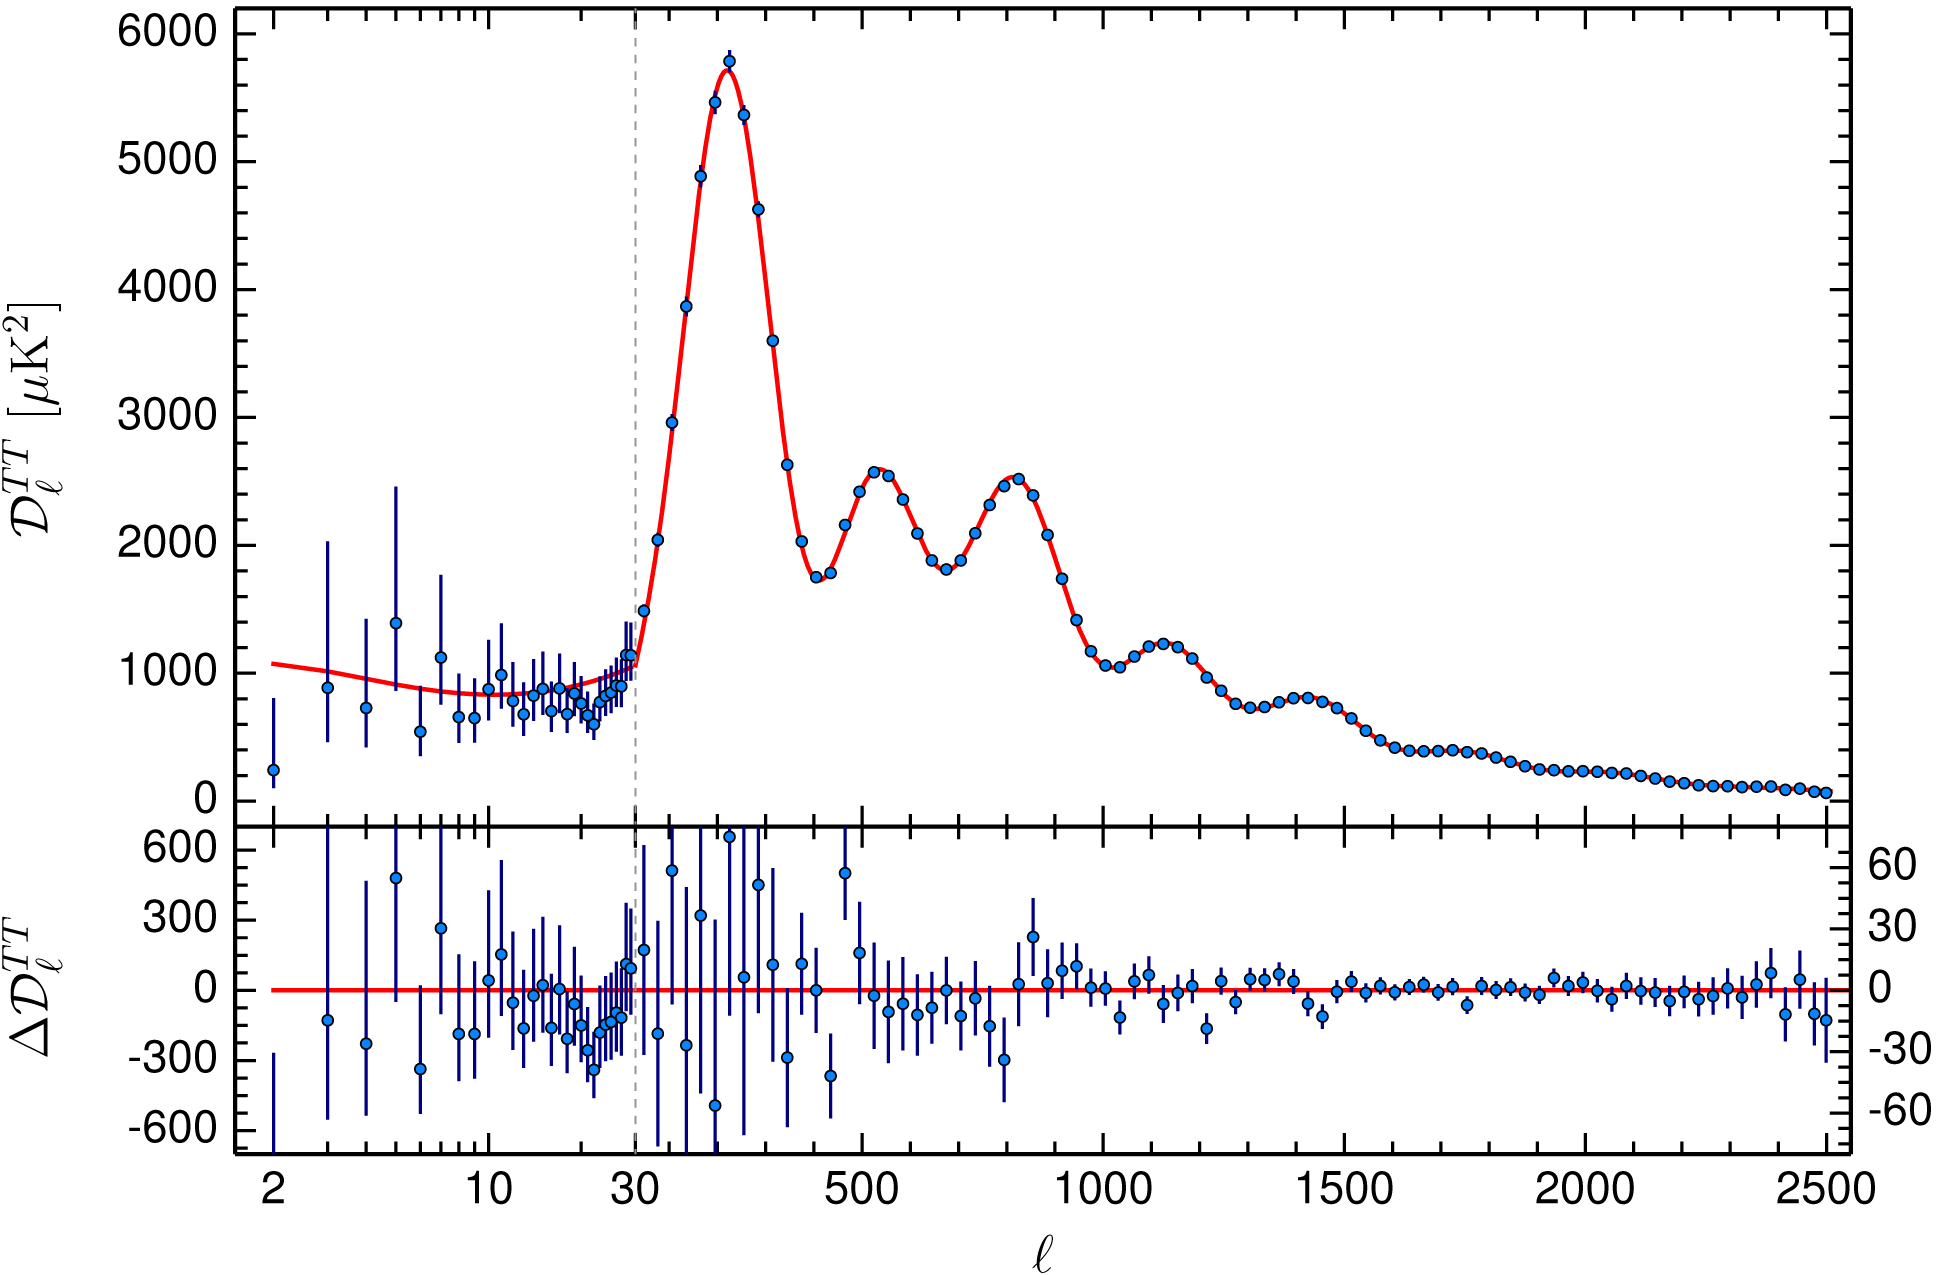
\includegraphics[width=\textwidth]{planck_aps}
        \caption{Plank angular power spectrum}
        \label{fig:planck_aps}
\end{figure}

For small values of $l$ we notice a plateau, caused by the Sachs-Wolfe
effect. At larger $l$, the spectrum exhibits a distinctive patterns of
patterns of peaks and troughs, an evidence of acoustic oscillation in the
early Universe.

Data in the graph are well fitted by the standard
$\Lambda$CMD model. The main cosmological parameters defining this model of
the Universe are:

\begin{itemize}
        \item \textbf{Hubble constant:} it describes the expansion rate of
        the Universe at present time. The value obtained from Planck
        measures is

        \begin{equation}
                H_0 = \SI{67.8 \pm 0.9}{\kilo\meter\per\second\per\mega\parsec}.
        \end{equation}

        \item \textbf{Acoustic scale:} it is the characteristic angular
        scale of the fluctuations in CMB. This parameter is constrained by
        the position of the acoustic peaks. Plank observations yielded

        \begin{equation}
                \theta_* = \ang{0.59636 \pm 0.00025}.
        \end{equation}

        \item \textbf{Baryonic matter density:} the matter density
        parameters can be extracted from the relative heights of the
        acoustic peaks. The value for baryons has been determined to be

        \begin{equation}
                \Omega_b h^2 = \num{0.02222 \pm 0.00023}
        \end{equation}

        where $h$ is defined by

        \begin{equation}
                H_0 \equiv \SI{100}{\hubble\kilo\meter\per\second\per\mega\parsec}
        \end{equation}

        \item \textbf{Dark matter density:} the value of the dark matter
        density parameter is

        \begin{equation}
                \Omega_c h^2 = \num{0.1197 \pm 0.0022}.
        \end{equation}

        \item \textbf{Dark energy density:} The value of the dark energy
        density parameter is estimated to be

        \begin{equation}
                \Omega_\Lambda = \num{0.685 \pm 0.012}.
        \end{equation}

        \item \textbf{Spectral index:} The inflationary paradigm predicts
        the power spectrum of primordial density perturbations to be a
        power law,

        \begin{equation}
                P\qty(\vb{k},t = t_\text{BigBang}) = k^n.
        \end{equation}
        The index $n$, which is known as the spectral index, has the
        following value:

        \begin{equation}
                n = \num{0.9655 \pm 0.0062}.
        \end{equation}

        \item small-scale fluctuation in the CMB are damped by Thomson
        scattering from free electrons produced during reionization. Modes
        with wavelength smaller than the apparent horizon at reionization
        was suppressed by a factor $e^{-2\tau}$, where $\tau$ is the optical
        depth of Thomson scattering. The resulting value of $\tau$ from Planck
        temperature power spectrum is

        \begin{equation}
                \tau = \num{0.078 \pm 0.019}.
        \end{equation}
\end{itemize}

\section{The Inflationary Paradigm}

The $\Lambda$CDM cosmological model describes very well some of the
cosmological observations, in particular the presence of the CMB black
body radiation and the abundance of light elements in the Universe.
Netherless, some fact about our Universe linger unexplained.

\subsection{Open Issues of the Big Bang Cosmology}\label{ss:issues}

The three fundamental issue unsolved by the Big Bang model follow:

\begin{itemize}
        \item \textbf{Horizon problem:} observations of the cosmic
        microwave background radiation shows that our Universe is very
        homogeneous and isotropic on the largest scales. In particular we
        know that zones of the Universe sitting at distance larger than the
        horizon during recombination and, for this reason, not causally
        connected, are characterized by the same CMB temperature.
        In fact, regions that in the standard Big Bang model would be causally
        connected at the time of the last scattering, subtend today an
        angle of \ang{\sim 1} in the sky.

        \item \textbf{Flatness problem:} current observations show a very
        flat universe, but the solutions of Friedmann equations for a
        radiation dominated universe describes flat curvature as a rather
        unstable condition. To explain the current spatially flat geometry
        we need to introduce ad hoc initial conditions in the model.

        \item \textbf{Initial conditions problem:} the Big Bang model
        does not furnish a physical mechanism to introduce density
        fluctuations in the early Universe. The presence of primordial
        fluctuations is required to explain the formation of galaxies and
        clusters we observe today.
\end{itemize}

\subsection{Inflation}

The issues presented in \autoref{ss:issues} can be solved introducing a
phase of accelerated expansion in the early universe, between
\SIlist{e-36;e-34}{\second} after the Big Bang. This idea is known as
\emph{inflation} or \emph{inflationary paradigm} and it was introduces by
Alan Guth in 1981.

\subsection{A Solution to Flatness and Horizon Problems}

To understand how inflation can solve the issues left unsolved by the Big Bang
model, we first define some useful quantities: the \emph{comoving particle
horizon} and the \emph{comoving apparent horizon}.

The comoving particle horizon is defined as

\begin{equation}
        \chi_H\qty(t) \equiv \int^t_0 \frac{c\dd{t'}}{a\qty(t')} =
        \int^a_0 \frac{\dd{a}}{a} \frac{c}{a\qty(t) H\qty(t)}
        \label{eq:horizons}
\end{equation}

and the quantity $d_{H,\text{co}}\qty(t) = c/a\qty(t)H\qty(t)$, which
appears in the second integral is the comoving apparent horizon.

If particles are separated by a comoving distance greater than
$\chi_H\qty(t)$ at a certain time $t$, they could not have been in causal
connection in the past. In turn, if the separating distance is more than
$d_{H,\text{co}}$, the two particles can not communicate \emph{now}. It is
possible that $\chi_H\qty(t)$ is much larger than $d_{H,\text{co}}$ now,
so that certain particles in the Universe cannot communicate at present
time, but were in causal contact early on. We see from \autoref{eq:horizons}
that the condition for this to happen is a comoving apparent horizon much larger
in the early Universe than now. Hence a phase of decreasing comoving
apparent horizon is required.

A decreasing comoving apparent horizon means that scale of the CMB
radiation entering the horizon at present time were inside the comoving
apparent horizon during inflation (see \autoref{fig:horizon_inflation_solution}).
In other words, they are inside the comoving particle horizon. That is
enough to solve the horizon problem.

\begin{figure}
        \centering
        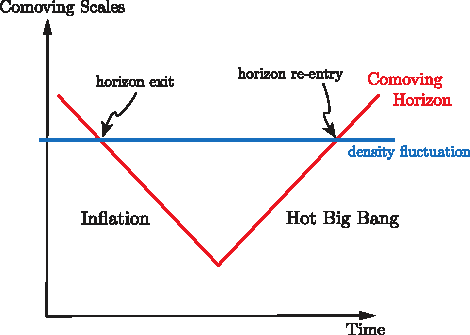
\includegraphics[width=0.9\textwidth]{horizon_inflation_solution}
        \caption{Solution for the inflationary problem (forse la prendo
        dalle dispense sull'inflazione)}
        \label{fig:horizon_inflation_solution}
\end{figure}


We can understand how the flatness problem is solved rewriting
\autoref{eq:friedmann_curvature} in term of the comoving apparent horizon
and taking its absolute value.  We obtain

\begin{equation}
        \abs{\Omega\qty(t) - 1} = k d_{H,\text{co}}.
\end{equation}

If the comoving apparent horizon decreases the Universe is driven toward
flatness. The solution $\Omega = 1$ is an attractor during inflation.

\subsection{Conditions for Inflation}

We have just seen that the a necessary condition for inflation is a
shrinking comoving apparent horizon in the early Universe. This is
equivalent to

\begin{equation}
        \dot d_{H,\text{co}} < 0.
\end{equation}

Calculation of the time derivative yields

\begin{equation}
        \frac{-\ddot a\qty(t)}{a^2\qty(t) H^2\qty(t)} < 0
\end{equation}

therefore a necessary condition for inflation is a phase of accelerated
expansion of the Universe,

\begin{equation}
        \ddot a\qty(t) > 0
\end{equation}

The second time derivative of the scale factor can be related to the first
time derivative of the Hubble parameter in this way

\begin{equation}
        \frac{\ddot a\qty(t)}{a\qty(t)} = H^2\qty(t)\qty(1 - \epsilon\qty(t)).
\end{equation}

$\epsilon$ is known as the \emph{slow-roll parameter} and is defined as
$\epsilon\qty(t) \equiv -\dot H\qty(t)/H^2\qty(t)$.
Therefore, for an accelerating phase to happen in the early universe is
required that

\begin{equation}
        \epsilon\qty(t) < 1.
\end{equation}

This condition implies that the fractional change of the Hubble parameter
is small during inflation. As a result we can assume

\begin{equation}
        H\qty(t) = H_I = \text{const.}
\end{equation}

during inflation.

Furthermore, looking at the second Friedmann equation, we infer that the condition $\ddot
a > 0$ requires

\begin{equation}
        P\qty(t) < -\frac{1}{3} \rho\qty(t).
\end{equation}

This demands the presence of a component of the cosmological fluid
characterized by the negative pressure, or, in an equivalent way, a
violation of the \emph{strong energy condition}.

\subsection{Physics of Inflation}

A simple physical model of inflation involves a single scalar field
$\phi\qty(\vb{\chi},t)$, known as \emph{inflaton}. The physical nature of
the inflaton is unknown, but we can simply use it as an \emph{order
paramerer} to parametrize the time-evolution of the inflationary energy
density.

The action associated to the a scalar field weakly coupled to gravity is

\begin{equation}
        S\qty[g,\phi] = S_{EH}\qty[g] + S_\phi\qty[g,\phi]
\end{equation}

where $S_{EH}\qty[g]$ is the gravitational Einstein-Hilbert action and
$S[g,\phi]$ is generic action for a scalar field. The explicit shapes of
these action action terms are

\begin{align}
        S_{EH}[g] & = \frac{1}{16\pi G} \int \sqrt{-g} R \dd[4]{\chi} \\
        S_\phi[g,\phi] & = \frac{\sqrt{-g}}{2}
        g^{\mu \nu}\partial_\mu\phi\partial_\nu\phi - V\qty(\phi)
\end{align}

where $V\qty(\phi)$ is a potential that describes the self-interactions of
the scalar field $\phi$.

The application of the variational principle to the action gives the
field equation of motion

\begin{equation}
        \frac{1}{\sqrt{-g}} \partial_\mu\qty(\sqrt{-g} \partial^\mu\phi) +
        V'\qty(\phi) = 0
\end{equation}

Assuming the FLRW metric for $g_{\mu \nu}$ and that we are working with an
homogeneous field $\phi\qty(\vb{\chi},t) \equiv \phi\qty(t)$, the equation
of motion become

\begin{equation}
        \ddot \phi + 3H \dot\phi + V'\qty(\phi) = 0
\end{equation}

the equation of motion of a damped harmonic oscillator and the field
evolves towards the minimum potential condition.

Under the same assumptions the energy momentum tensor of the field takes
the form of a perfect fluid, with the following pression and density,

\begin{align}
        \rho_\phi c^2 & = \frac{1}{2} \dot\phi^2 + V\qty(\phi) \\
        P_\phi & = \frac{1}{2}\dot\phi^2 - V\qty(\phi).
\end{align}

The usual $w$ proportionality parameter in the scalar field state equation
is

\begin{equation}
        w_\phi\qty(t) = \frac{\frac{1}{2} \dot\phi^2 - V\qty(\phi)}{\frac{1}{2}
        \dot\phi^2 + V\qty(\phi)}
\end{equation}

So in this case the slow-roll parameter becomes

\begin{equation}
        \epsilon\qty(t) \equiv \frac{3}{2} \qty(w_\phi\qty(t) + 1) =
        \frac{1}{2} \frac{\dot\phi^2\qty(t)}{H^2\qty(t)}
\end{equation}

Accelerated expansion takes place when $\epsilon\qty(t) < 1$. In particular
in the case limit defined by

\begin{equation}
        \dot\phi^2 \ll V\qty(\phi)
        \label{eq:sr_condition_1}
\end{equation}

$\epsilon\qty(t) \ll 1$, so as previously stated $H\qty(t) = H_I =
\text{const.}$ and we are in the de Sitter limit,

\begin{equation}
        P_\phi\qty(t) \approx -\rho_\phi\qty(t)
\end{equation}

that is, the inflaton behaves like a perfect fluid characterized by
negative pressure, as in the case of Dark Energy.

Accelerated expansion is sustained for a sufficiently long period of time
only if $\ddot \phi\qty(t)$ is small enough,

\begin{equation}
        \abs{\ddot\phi} \ll \abs{3H\dot\phi}, \abs{V'\qty(\phi)}.
        \label{eq:sr_condition_2}
\end{equation}

\autoref{eq:sr_condition_1} and \autoref{eq:sr_condition_2} are known as
\emph{slow-roll conditions}. Under them the equation of motion for the
scalar inflation field and the first Friedmann equation become

\begin{align}
        \dot\phi \approx & -\frac{V'\qty(\phi)}{3H}  \\
        H^2 \approx & \frac{8\pi G}{3} V\qty(\phi) = H_I
\end{align}

From the last equation we understand that during inflation the spacetime is
approximately de Sitter with the scale factor undergoing exponential growth,

\begin{equation}
        a\qty(t) \approx a\qty(t_I)e^{H_I\qty(t - t_I)}
\end{equation}

as expected. The inflation epoch comes to an end when thw slow-roll
conditions are violated,

\begin{equation}
        \epsilon(t_{I,\text{end}}) \equiv 1,
\end{equation}

from that time on the inflation field kinetic energy starts to grow,
until the field potential comes to its minimum. The field energy is
dissipated in a process called \emph{reheating} and an epoch well
described by standard cosmology follows.

There are different inflaton potentials that guarantees slow-roll
conditions and each one of them corresponds to a distinct model of
inflation. An example of inflaton potential is shown in
\autoref{fig:inflaton_potential}.

\begin{figure}
        \centering
        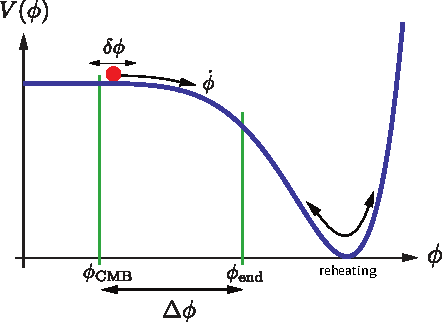
\includegraphics[width=\textwidth]{inflaton_potential}
        \caption{Example of inflaton potential}
        \label{fig:inflaton_potential}
\end{figure}

\subsection{Inflation and Primordial Perturbations}

The inflationary paradigm can also solve the initial conditions problem,
providing a physical mechanism to introduce perturbations in the early
universe. The non-uniformity arises from quantum fluctuations in the
inflaton field, which appear as linear perturbations of the field itself.

The Universe at the time of inflation was dominated by the inflation field,
therefore scalar, vector and tensor first order perturbations arose in
the spacetime metric. The three kind of perturbations evolve independently:
vector perturbations decay in an expanding universe. Instead, scalar and
tensor perturbations exhibit the following power spectra:

\begin{align}
        P_\phi & \propto k^{n_S - 4} \\
        P_h & \propto k^{n_T - 3}
\end{align}

respectively. The predicted values of the spectral
indices are, $n_S \approx 1$ and $n_T \approx 0$.
Matter density fluctuations in the primodial Universe developed from
scalar perturbations of the metric. On the other hand, tensor perturbations
of the metric caused propagation of \emph{primordial gravitational waves}
(PGW) in the early Universe. The \emph{tensor-to-scalar ratio}, $r$, represents
the relative amplitude of tensor perturbations as compared to the amplitude
of scalar perturbations:

\begin{equation}
        r \equiv \frac{P_h}{P_\phi} \propto \epsilon.
\end{equation}

We have already stated that during the \emph{slow-roll} phase $\epsilon \ll
1$, thus the inflationary paradigm predicts the presence of primordial
gravitatiol waves, whose amplitude is much smaller than the amplitude of
temperature anisotropies. Moreover, the slow roll parameter, and thus the
tensor-to-scalar ratio, depends on the specific shape of the inflation
potential, $V\qty(\phi)$. Therefore different inflationary models predict
different amplitudes for primordial gravitational waves. In any case, the
presence of primordial gravitational waves constitutes a \emph{smoking gun} in favor
of inflation. Indirect evidence of the presence of such early perturbations of
the spacetime metric is cointained in the polarization of the cosmic microwave
background radiation.

\section{The CMB Polarization}

Polarization in the cosmic microwave background was generated through
Thomson scattering events occurred during recombination. The total
scattering cross section of an incoming unpolarized radiation by an
electron is given by

\begin{equation}
        \dv{\sigma}{\Omega} = \frac{3\sigma_T}{8\pi}
        \abs{\vectorunit{\epsilon}' \vdot \vectorunit{\epsilon}}
        \label{eq:thomson_csection}
\end{equation}

where $\sigma_T$ is the total Thomson scattering cross-section and the unit
vectors $\vectorunit{\epsilon}$ and $\vectorunit{\epsilon}'$ lie in the
plane perpendicular to the propagation direction of the incident radiation
and are parallel to the scattered and incident polarization, respectively.

\subsection{The Stokes Parameters}

To understand under what conditions the outgoing radiation of a Thomson
scattering event can be linearly polarized, it is convenient to introduce the
Stokes parameters. Consider a monochromatic plane electromagnetic wave
propagating in the $\vectorunit{z}$ direction. The field components are

\begin{align}
        E_x\qty(t) & = a_x\qty(t)\cos(\omega t - \phi_x) \\
        E_y\qty(t) & = a_y\qty(t)\sin(\omega t - \phi_y).
\end{align}

If some correlation exists between the two components, the radiation is
polarized.

The Stoke parameters are defined as the following time averages:

\begin{align}
        I & \equiv \expval{a^2_x\qty(t)} + \expval{a^2_y\qty(t)} \\
        Q & \equiv \expval{a^2_x\qty(t)} - \expval{a^2_y\qty(t)} \\
        U & \equiv \expval{2a_x\qty(t)a_y\qty(t)
        \cos(\theta_x\qty(t) - \theta_y\qty(t))} \\
        V & \equiv \expval{2a_x\qty(t)a_y\qty(t)
        \sin(\theta_x\qty(t) - \theta_y\qty(t))}
\end{align}

The parameter $I$ gives the intensity of the radiation, which corresponds
to the black body radiation intensity. The other parameters, $Q$, $U$ and
$V$ describes linear and circular polarization, respectively. The CMB
radiation is not circularly polarized, therefore in the following
dissertation we assume $V = 0$. I is a scalar quantity and does not depend
on the frame reference system. Instead, $Q$ and $U$ depend on the
orientation of the x and y axis.

$Q$ and $U$ parameters, undergoing a rotation of the $x$-$y$ plane through
an angle $\theta$, transform as

\begin{align}
        Q' & = Q\cos{2\theta} + U\sin{2\theta} \\
        U' & = -Q\sin{2\theta} + U\cos{2\theta}.
\end{align}

This transformation is characteristic of the second rank tensor:

\begin{equation}
        P = \frac{1}{2} \mqty(Q & U \\
                              U & -Q)
\end{equation}

An object invariant under an axis rotation through an angle of $\pi$.

If now we consider a monochromatic unpolarized incident plane wave of
intensity $I'$ and cross sectional area $\sigma_B$, which is scattered in
the $z$-axis direction, with the $y$-axis laying in the scattering plane,
the $Q$ and $U$ Stokes parameters of the outgoing radiation follow from
\autoref{eq:thomson_csection}:

\begin{align}
        Q\qty(\theta) & = \frac{3\sigma_T}{8\pi\sigma_B}I'\sin^2\theta
        \label{eq:q_thomson_mono} \\
        U\qty(\theta) & = 0 \label{eq:u_thomson_mono}
\end{align}

where $\theta$ is the angle between the outgoing and incoming wave.

In the case of a generic incoming radiation field of intensity $I' =
I\qty(\theta,\phi)$ we can perform an integration of
\autoref{eq:q_thomson_mono} and \autoref{eq:u_thomson_mono} over all
spatial directions, rotating all incoming to waves, so that the Stokes
parameters for the outgoing radiation are defined with respect to a common
frame reference system. The result, expressed in terms of the spin-2 object
$Q - iU$, is

\begin{equation}
        (Q -iU)\qty(\vectorunit{z}) = \frac{3\sigma_T}{16\pi \sigma_B}
        \int \dd{\Omega} \sin^2\theta e^{2i\phi}I'\qty(\theta,\phi)i.
\end{equation}

The incoming radiation field can be expanded in spherical harmonics as
usual:

\begin{equation}
        I'\qty(\theta,\phi) = \sum^\infty_{l = 0}\sum^l_{m = -l}
        a_{l,m} Y_{l,m}\qty(\theta,\phi).
\end{equation}

As a result, the linear polarization Stokes parameters become

\begin{equation}
        (Q - iU)\qty(\vectorunit{z}) = \frac{3\sigma_T}{4\pi\sigma_B}
        \sqrt{\frac{2\pi}{15}} a_{2,2}.
\end{equation}

Consequently, linear polarization is generated provided that the \emph{quadrupole
moment} of the incoming radiation is non-zero. This result is illustrated
in \autoref{fig:thomson_scattering}.

\begin{figure}
        \centering
        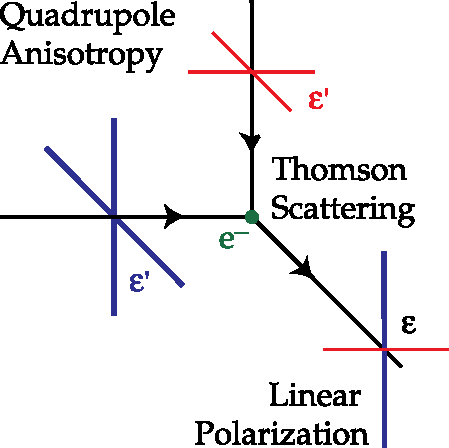
\includegraphics[width=0.64\textwidth]{thomson_scattering}
        \caption{Thomson scattering of quadrupole temperature anisotropies.
        (A CMB polarization primer)}
        \label{fig:thomson_scattering}
\end{figure}

Quadrupole anisotropies before recombination are rapidly damped away,
because photons are strongly coupled with electrons in primordial plasma, so
radiation can only posses a monopole and a dipole, corresponding to Doppler
shift from peculiar velocity. A quadrupole moment is produced only
\emph{during} recombination, as the mean free path of photons increases and
reaches the appropriate length scale.

\subsection{The Polarization Angular Power Spectrum}

As anticipated in the previous section the Stokes polarization parameters
$Q$ and $U$ transform under rotations and in particular the quantity $Q \pm
iU$ transform like a spin-2 object, therefore we can expand them in terms
of \emph{tensor spherical harmonics}:

\begin{equation}
        (Q \pm iU)\qty(\theta,\phi) = \sum^\infty_{l=0}\sum^l_{m=-l}
        a^{\qty(\pm 2)}_{l,m} Y^{\qty(\pm 2)}_{l,m}\qty(\theta,\phi)
\end{equation}

where $Y^{\qty(\pm 2)}_{l,m}$ and $a^{\qty(\pm 2)}_{l,m}$ are complex
coefficients.

It is convenient to define the following linear combination of the spin-2
coefficients:

\begin{align}
        a^{\qty(E)}_{l,m} & \equiv -\frac{a^{\qty(2)}_{l,m} + a^{\qty(-2)}_{l,m}}
        {2} \\
        a^{\qty(B)}_{l,m} & \equiv \frac{i}{2}
        \frac{a^{\qty(2)}_{l,m} - a^{\qty(-2)}_{l,m}}{2},
\end{align}

whose behavior under parity transformation is

\begin{align}
        a^{\qty(E)}_{l,m} & \rightarrow \qty(-1)^l a^{\qty(E)}_{l,m} \\
        a^{\qty(B)}_{l,m} & \rightarrow \qty(-1)^{l + 1} a^{\qty(B)}_{l,m}
\end{align}

Starting from this coefficients we can define the two quantities:

\begin{align}
        E\qty(\theta,\phi) & = \sum^\infty_{l=0}\sum^l_{m=-l}
        a^{\qty(E)}_{l,m} Y_{l,m}\qty(\theta,\phi) \\
        B\qty(\theta,\phi) & = \sum^\infty_{l=0}\sum^l_{m=-l}
        a^{\qty(B)}_{l,m} Y_{l,m}\qty(\theta,\phi).
\end{align}

the scalar fields $E\qty(\theta,\phi)$ and $B\qty(\theta,\phi)$ completely
specify all the statististical properties of the linear polarization
field. They are known as the \emph{E-modes} and \emph{B-modes} of the
cosmic microwave background and, like the $a^{\qty(E)}_{l,m}$ and
$a^{\qty(B)}_{l,m}$ coefficients, behaves differently under parity
transformation, as illustrated in \autoref{fig:eb_modes_patterns}

\begin{figure}
        \centering
        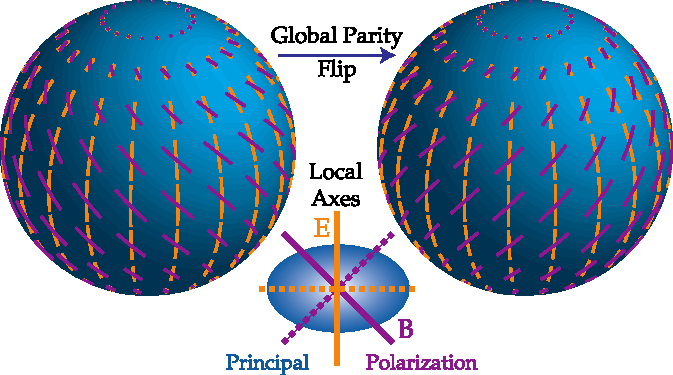
\includegraphics[width=0.9\textwidth]{eb_modes_patterns}
        \caption{E- and B-modes patterns (CMB polarization primer)}
        \label{fig:eb_modes_patterns}.
\end{figure}

To extract information from polarization measures of the CMB, we can employ
a statistical approach as we have previously done for CMB temperature anisotropies.
For this purpose, it is useful to compute the correlation and cross-correlation
function or, in an equivalent way, the auto- and cross-correlation power
spectra:

\begin{align}
        C^{TT}_l & = \frac{1}{2l + 1}\sum_m
        a^{\qty(T)*}_{l,m} a^{\qty(T)}_{l,m} \\
        C^{EE}_l & = \frac{1}{2l + 1}\sum_m
        a^{\qty(E)*}_{l,m} a^{\qty(E)}_{l,m} \\
        C^{BB}_l & = \frac{1}{2l + 1}\sum_m
        a^{\qty(B)*}_{l,m} a^{\qty(B)}_{l,m} \\
        C^{TE}_l & = \frac{1}{2l + 1}\sum_m
        a^{\qty(T)*}_{l,m} a^{\qty(E)}_{l,m}.
\end{align}

There's no correlation between E-modes and B-modes, because they are
generated by different physical phenomena. The same holds for TB cross
correlation. The CMB power spectra predicted on the base of the
$\Lambda$CDM model are represented in
\autoref{fig:predicted_power_spectra}.

\begin{figure}
        \centering
        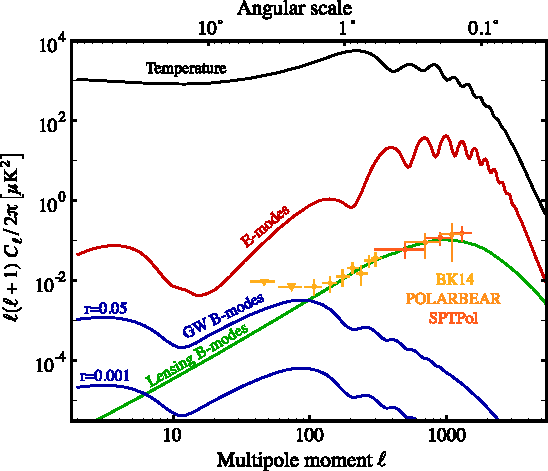
\includegraphics[width=\textwidth]{predicted_power_spectra}
        \caption{Predicted CMB power spectra}
        \label{fig:predicted_power_spectra}
\end{figure}

Quadrupole anisotropies can be decomposed into:

\begin{itemize}
        \item \textbf{Scalar perturbations:} $l = 2, m = 0$

        which are generated by density fluctuations in the primordial
        plasma. Thanks to Thomson scattering during recombination, they
        cause linear polarization in the CMB.

        \item \textbf{Vector perturbations:} $l = 2, m = \pm 1$

        which are caused by vortical motions of the matter. These kind of
        perturbations are damped by the expansion of the Universe, because
        they are associated to motions that are not enhanced by gravity.
        They are not expected to leave an imprint in the CMB radiation.

        \item \textbf{Tensor perturbation:} $l = 2, m = \pm 2$

        which can only be generated by perturbations of the metric in the
        early universe, in other words, gravitational waves that cause
        linear polarization in the CMB.
\end{itemize}

Therefore, the linear polarizations due to scalar and tensor perturbations was
generated by quadrupole anisotropies that were present only for a short time
interval, close to recombination epoch. So, we expect a faint signal compared to
that of the temperature anisotropies: \SI{\leq e-6}{\kelvin}.

\section{Foreground Contamination}
